%% LaTeX2e class for student theses
%% sections/results.tex
%% 
%% Karlsruhe Institute of Technology
%% Institute for Program Structures and Data Organization
%% Chair for Software Design and Quality (SDQ)
%%
%% Dr.-Ing. Erik Burger
%% burger@kit.edu
%%
%% Version 1.3.2, 2017-08-01

\chapter{Results}
\label{ch:Results}

The algorithm was analyzed from two different perspectives: EMS procedure detection, and generalizability. The machine learning algorithm analysis focuses on the algorithm’s ability to classify EMS procedures and generalize across populations. The algorithm analysis for CPR, Bag-Valve-Mask Ventilation, placing an oral airway, placing an IV tourniquet, and wrapping a head wound is presented first, followed by the task generalizability in Section \ref{sec:Results:Generalizability}.
\par The machine learning algorithms' ability to detect EMS procedures is analyzed using F1-Measure, precision, and recall value. The results are compared to three different machine learning algorithms: SVM, decision-tree, and $k$-NN. The generalizability is analyzed by training the algorithm with each participants data separately and comparing it to the results of the combined data.
\par The parameters of the machine learning algorithms are tuned to improve the accuracy. The decision-tree algorithm achieved the highest score using the following parameters:
\begin{itemize}
	\item \texttt{criterion='gini'}
	\item \texttt{splitter='best'}
	\item \texttt{max\_depth=None}
	\item \texttt{min\_samples\_split=2}
	\item \texttt{min\_samples\_leaf=1}
	\item \texttt{max\_leaf\_nodes=None}
\end{itemize}
The SVM algorithm achieved the highest score using the following parameters:
\begin{itemize}
	\item \texttt{kernel='rbf'}
	\item \texttt{C=0.01}
	\item \texttt{gamma=1000}
\end{itemize}
The $k$-NN algorithm achieved the highest score using the following parameters:
\begin{itemize}
	\item $k$=4
	\item \texttt{weights=uniform}
	\item \texttt{algorithm=auto}
\end{itemize}
The HMM algorithm achieved the highest score using the following parameters:
\begin{itemize}
	\item \texttt{DistributionModel=NormalDistribution}
	\item \texttt{n\_components=1}
	\item \texttt{algorithm='baum-welch'}
\end{itemize}
\par The window size initially set at 2 seconds is varied at 4 seconds, and 6 seconds to improve recognition for procedures with similar movements. The F1 score improved for all machine learning algorithms by an average of 5\% when setting the window size at 6 seconds.
\section{Cardiopulmonary Resuscitation}
\label{sec:Results:CPR}
The participants took an average of 56.69 seconds (St. Dev. = 3.76) to complete one round of the cardiopulmonary resuscitation procedure. The participants were able to complete two rounds within the one minute data collection of every procedure. The amount of datasets for the third day were seven per participant, resulting in a total of 70 datasets.
\par The CPR datasets includes several unique movement observed in graphs for the IMU and EMG sensor. The first unique movement when performing CPR are the 30 compressions, particularly in the IMU sensor as seen in Figure \ref{fig:1571imuday3cpr31}. The acceleration for both hands have sinusoidal peaks with the greatest magnitude on the X-axis, which is the up-and-down motion from the arms. During the compressions the orientation does not change, nor is there any significant observation in the EMG sensor. The second unique movement is giving the two breaths, as seen in the EMS sensor in Figure \ref{fig:1571emgday3cpr31}. The right hand has two spikes in the beginning of the procedure and again after half of the procedure. The spikes are visible in channel three, four, five, and seven of the EMG sensor. The right hand's orientation also shows two spikes where the two breaths are given. The left hand shows no significant acceleration, orientation, or EMG data.
\begin{figure}
	\centering
	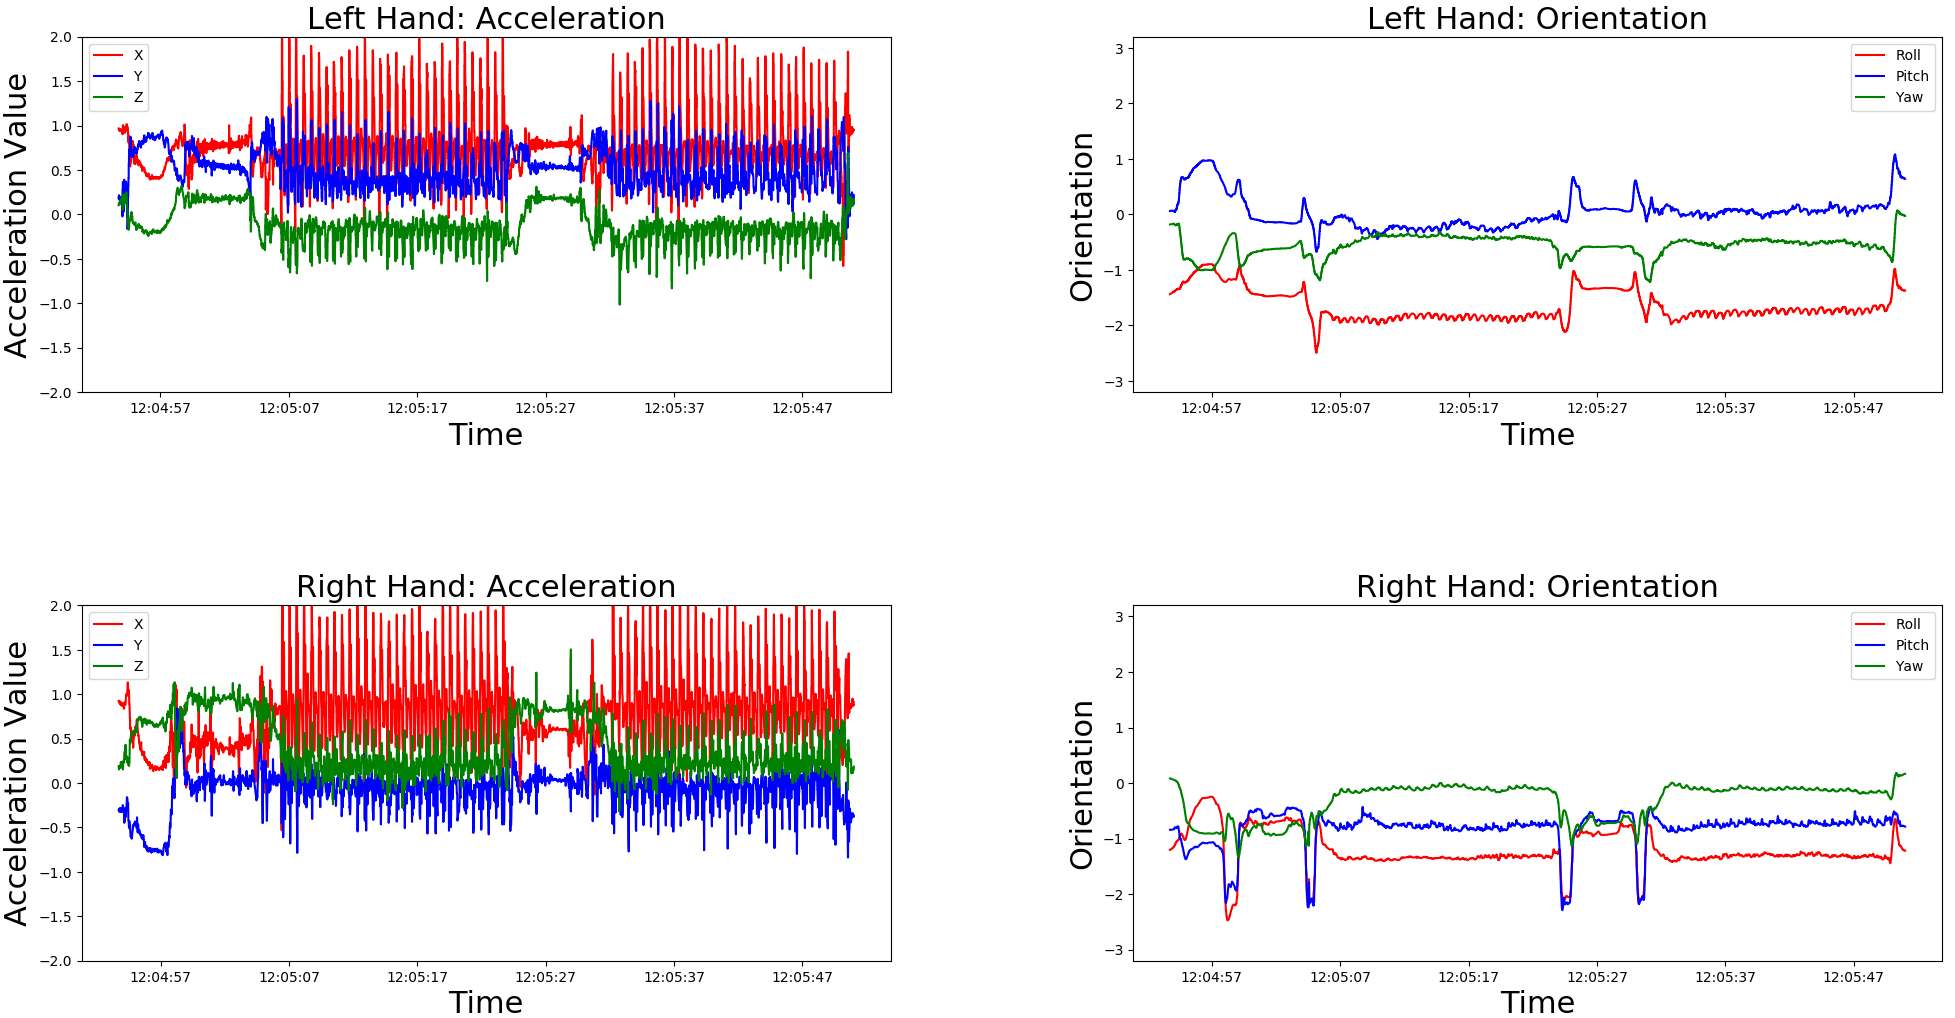
\includegraphics[width=0.8\linewidth]{pictures/1571_IMU_Day3_cpr_31}
	\caption{IMU data for CPR}
	\label{fig:1571imuday3cpr31}
\end{figure}
\begin{figure}
	\centering
	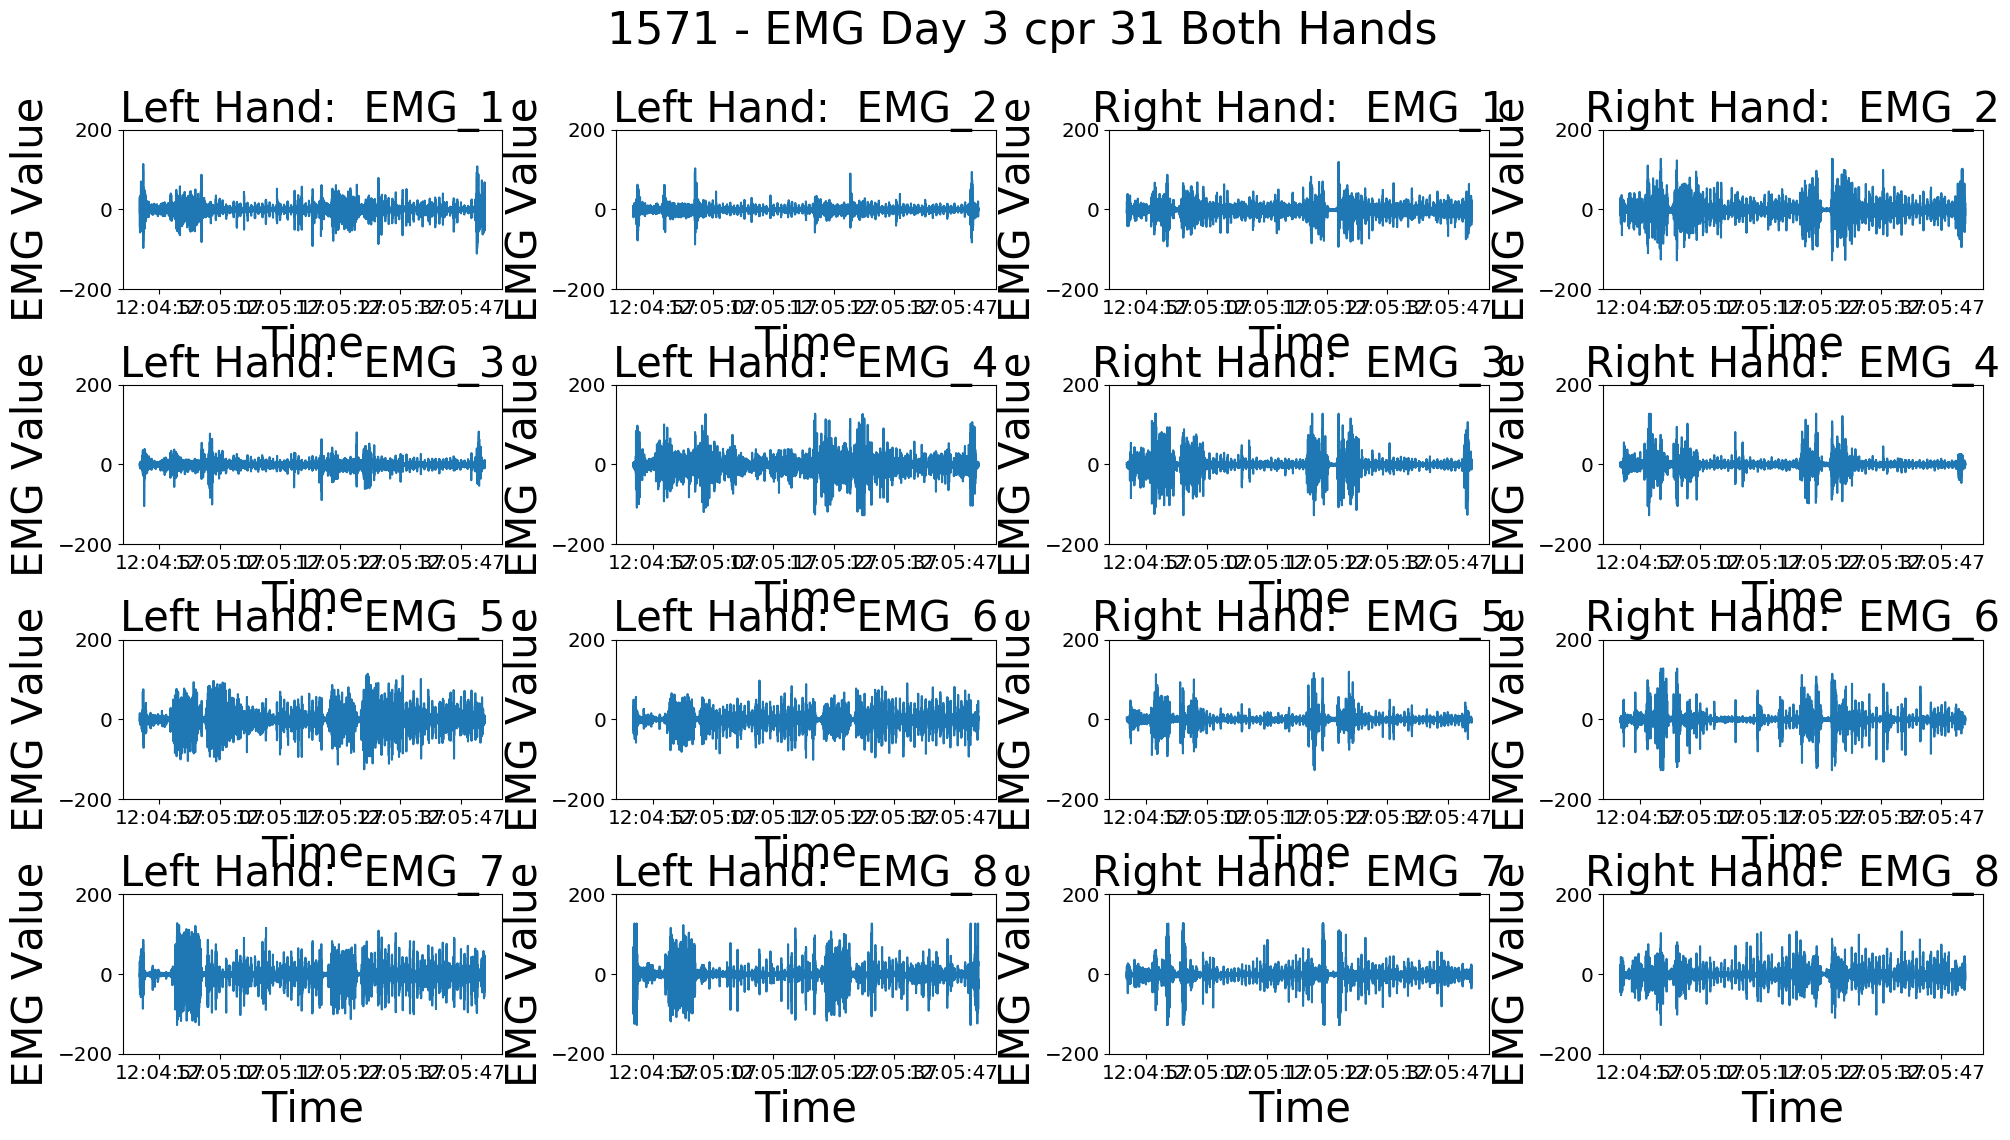
\includegraphics[width=0.8\linewidth]{pictures/1571_EMG_Day3_cpr_31}
	\caption{EMG data for CPR}
	\label{fig:1571emgday3cpr31}
\end{figure}
\par Each individual participant's datasets were used to train the decision-tree, SVM, $k$-NN, and HMM machine learning algorithms. The first participant had the lowest F1 score of all machine learning algorithms with 0.69 for the decision-tree, 0.31 for $k$-NN, 0.28 for SVM, 0.00 for HMM. The HMM had the highest standard deviation of 0.32 when recognizing CPR as shown in Table \ref{tab:cpr:ml}.
\newcommand*\rotv{\multirow{2}{*}{\rotatebox[origin=c]{45}}}
\begin{table}[]
	\centering
	\begin{tabular}{lllllllllllll}
		\multirow{2}{*}{\rotatebox[origin=c]{45}{\textbf{Participant}}} & \multicolumn{3}{c}{\textbf{decision-tree}} & \multicolumn{3}{c}{\textbf{$k$-NN} ($k=4$)} & \multicolumn{3}{c}{\textbf{SVM}} & \multicolumn{3}{c}{\textbf{HMM}} \\
		 & \rot{Precision}     & \rot{Recall}    & \rot{F1}    & \rot{Precision}     & \rot{Recall}    & \rot{F1}  & \rot{Precision}     & \rot{Recall}    & \rot{F1} & \rot{Precision}     & \rot{Recall}    & \rot{F1} \\
		\textbf{1}   & 0.69 & 0.69 & 0.69 & 0.37 & 0.27 & 0.31 & 0.37 & 0.22 & 0.28 & 0.00 & 0.00 & 0.00 \\
		\textbf{2}   & 0.85 & 0.83 & 0.84 & 0.36 & 0.19 & 0.25 & 0.42 & 0.36 & 0.39 & 0.44 & 0.67 & 0.53 \\
		\textbf{3}   & 0.84 & 0.81 & 0.82 & 0.41 & 0.24 & 0.31 & 0.42 & 0.37 & 0.39 & 0.40 & 0.33 & 0.36 \\
		\textbf{4}   & 0.84 & 0.86 & 0.85 & 0.54 & 0.33 & 0.41 & 0.55 & 0.47 & 0.51 & 0.42 & 0.83 & 0.56 \\
		\textbf{5}   & 0.81 & 0.82 & 0.82 & 0.66 & 0.37 & 0.47 & 0.66 & 0.50 & 0.57 & 0.29 & 0.67 & 0.40 \\
		\textbf{6}   & 0.78 & 0.80 & 0.79 & 0.36 & 0.16 & 0.22 & 0.40 & 0.34 & 0.37 & 0.36 & 0.67 & 0.47 \\
		\textbf{7}   & 0.89 & 0.91 & 0.90 & 0.55 & 0.44 & 0.49 & 0.68 & 0.53 & 0.60 & 0.38 & 1.00 & 0.55 \\
		\textbf{8}   & 0.89 & 0.90 & 0.89 & 0.22 & 0.09 & 0.13 & 0.42 & 0.37 & 0.40 & 0.12 & 0.17 & 0.14 \\
		\textbf{9}   & 0.90 & 0.87 & 0.88 & 0.49 & 0.23 & 0.31 & 0.61 & 0.47 & 0.53 & 0.50 & 0.83 & 0.62 \\
		\textbf{10} & 0.83 & 0.77 & 0.80 & 0.50 & 0.27 & 0.35 & 0.54 & 0.45 & 0.49 & 0.50 & 0.67 & 0.57 \\
		\hline
		\textbf{Mean} & 0.83 & 0.83 & 0.83 & 0.45 & 0.26 & 0.33 & 0.51 & 0.41 & 0.45 & 0.34 & 0.58 & 0.42 \\
		\textbf{Std. Dev.} & 0.06 & 0.07 & 0.06 & 0.13 & 0.10 & 0.11 & 0.12 & 0.09 & 0.10 & 0.16 & 0.32 & 0.20
	\end{tabular}
	\caption{Ten-fold cross validation for detecting CPR per participant}
	\label{tab:cpr:ml}
\end{table}
\subsection{Discussion}
\label{sec:Results:CPR:Discussion}
Contrary to the initial assumption, the unique movements during CPR were not as helpful to accuracy detect the procedure as predicted. The overlap of the giving breaths motion resulted in high misclassification as Bag-Valve-Mask ventilation.
\section{Bag-Valve-Mask Ventilation}
\label{sec:Results:BVM}
The participants took an average of 35.39 seconds (St. Dev. = 5.70) to complete one round of the Bag-Valve-Mask ventilation procedure. The participants were able to complete two rounds within the one minute data collection of every procedure. The amount of datasets for the third day were seven per participant, resulting in a total of 70 datasets.
\par The bag-valve-mask ventilation datasets consists of the unique squeezing motion in the EMG sensor graph. The sinusoidal motion is visible in all eight EMG channels in Figure \ref{fig:7073emgday3b46}. The squeezing motion of the right hand on the bag and the resting position of the left hand on the mask results in little movement of the IMU data. Figure \ref{fig:7073imuday3b46} shows almost flat lines for acceleration and orientation of both hands.
\par Bag-Valve-Mask ventilation achieved the lowest F1 scores of all procedures with F1 scores as low as 0.08, as seen in Table \ref{tab:bvm:ml}. The HMM classifier was the algorithm with the highest mean F1 score at 0.64 (Std. Dev=0.19), followed by the decision-tree algorithm at 0.60 (Std. Dev=0.09).
\begin{figure}
	\centering
	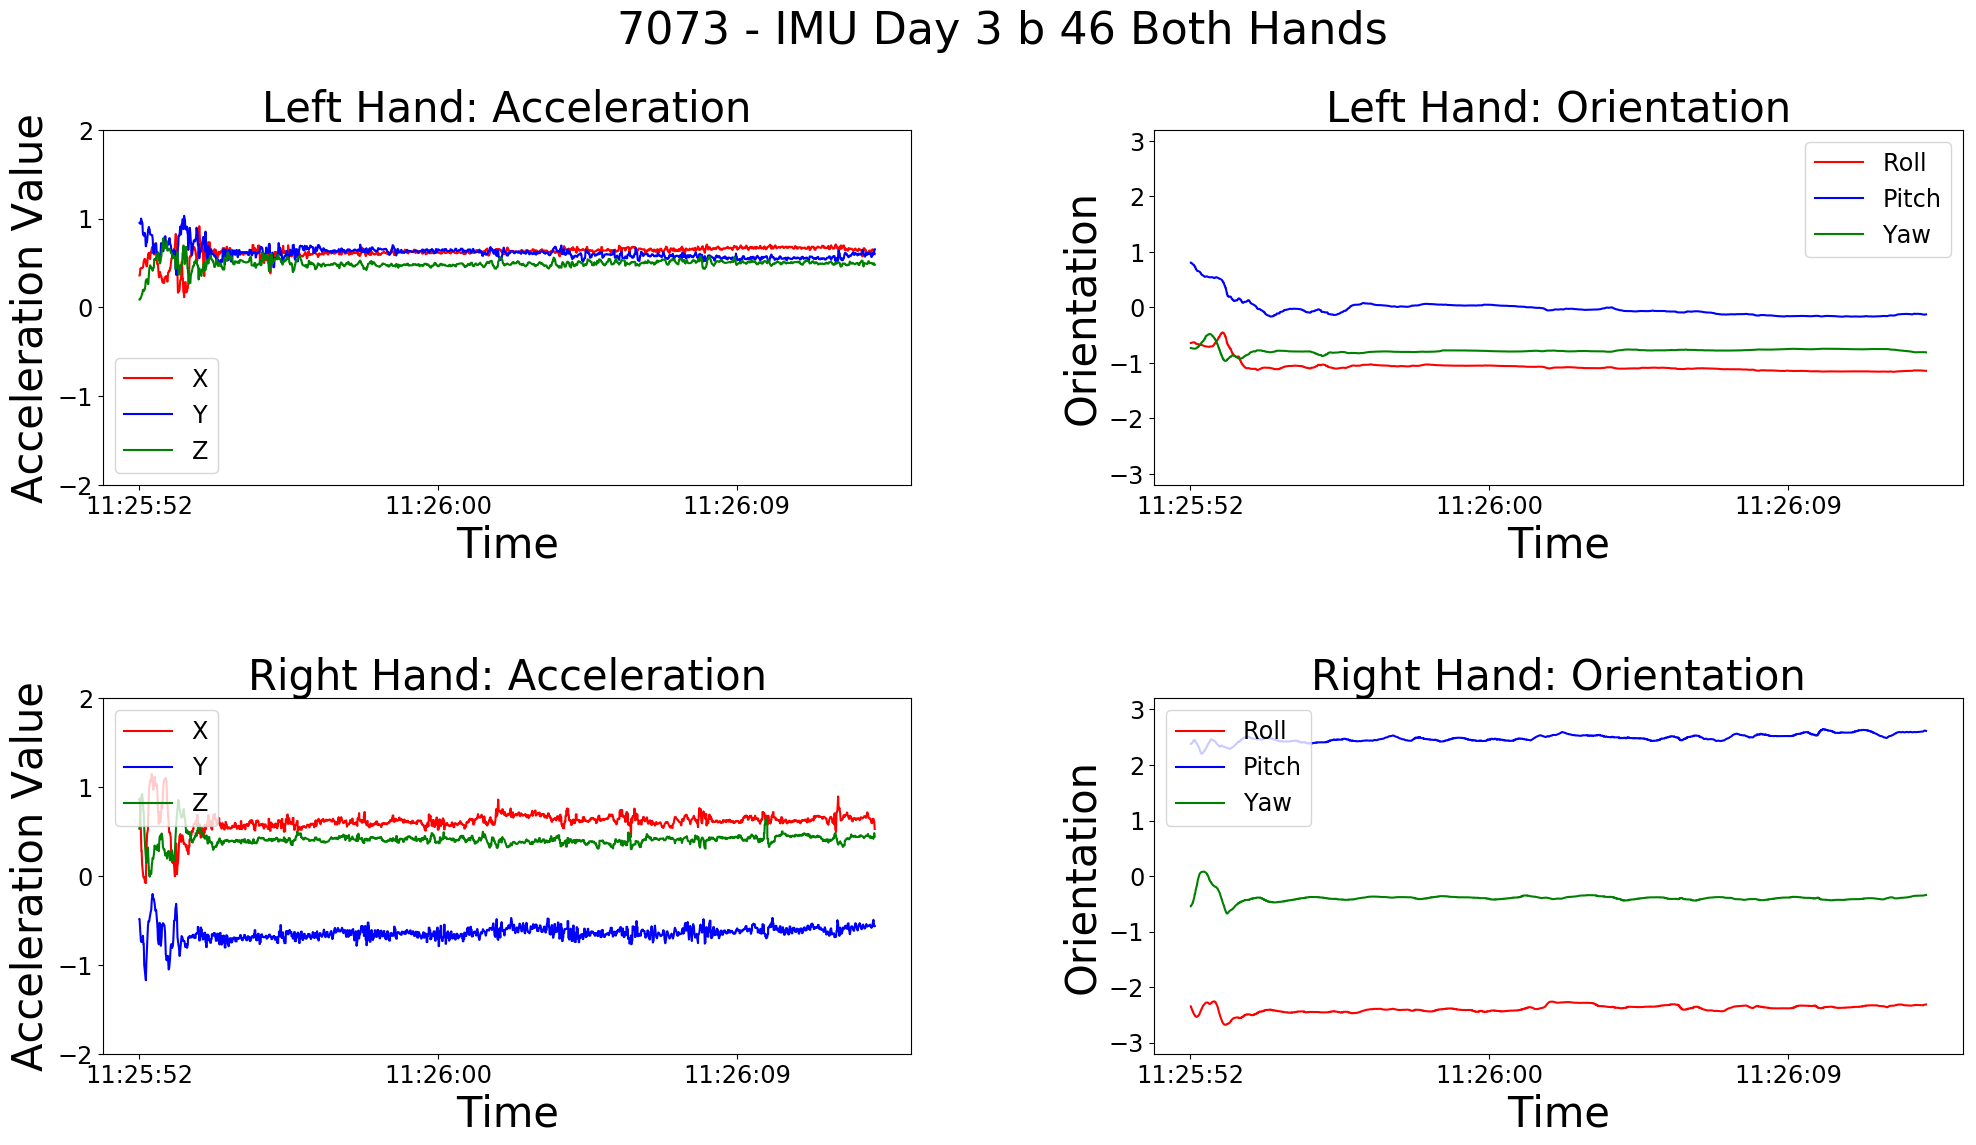
\includegraphics[width=0.8\linewidth]{pictures/7073_IMU_Day3_b_46}
	\caption{IMU data for Bag-Valve-Mask ventilation}
	\label{fig:7073imuday3b46}
\end{figure}
\begin{figure}
	\centering
	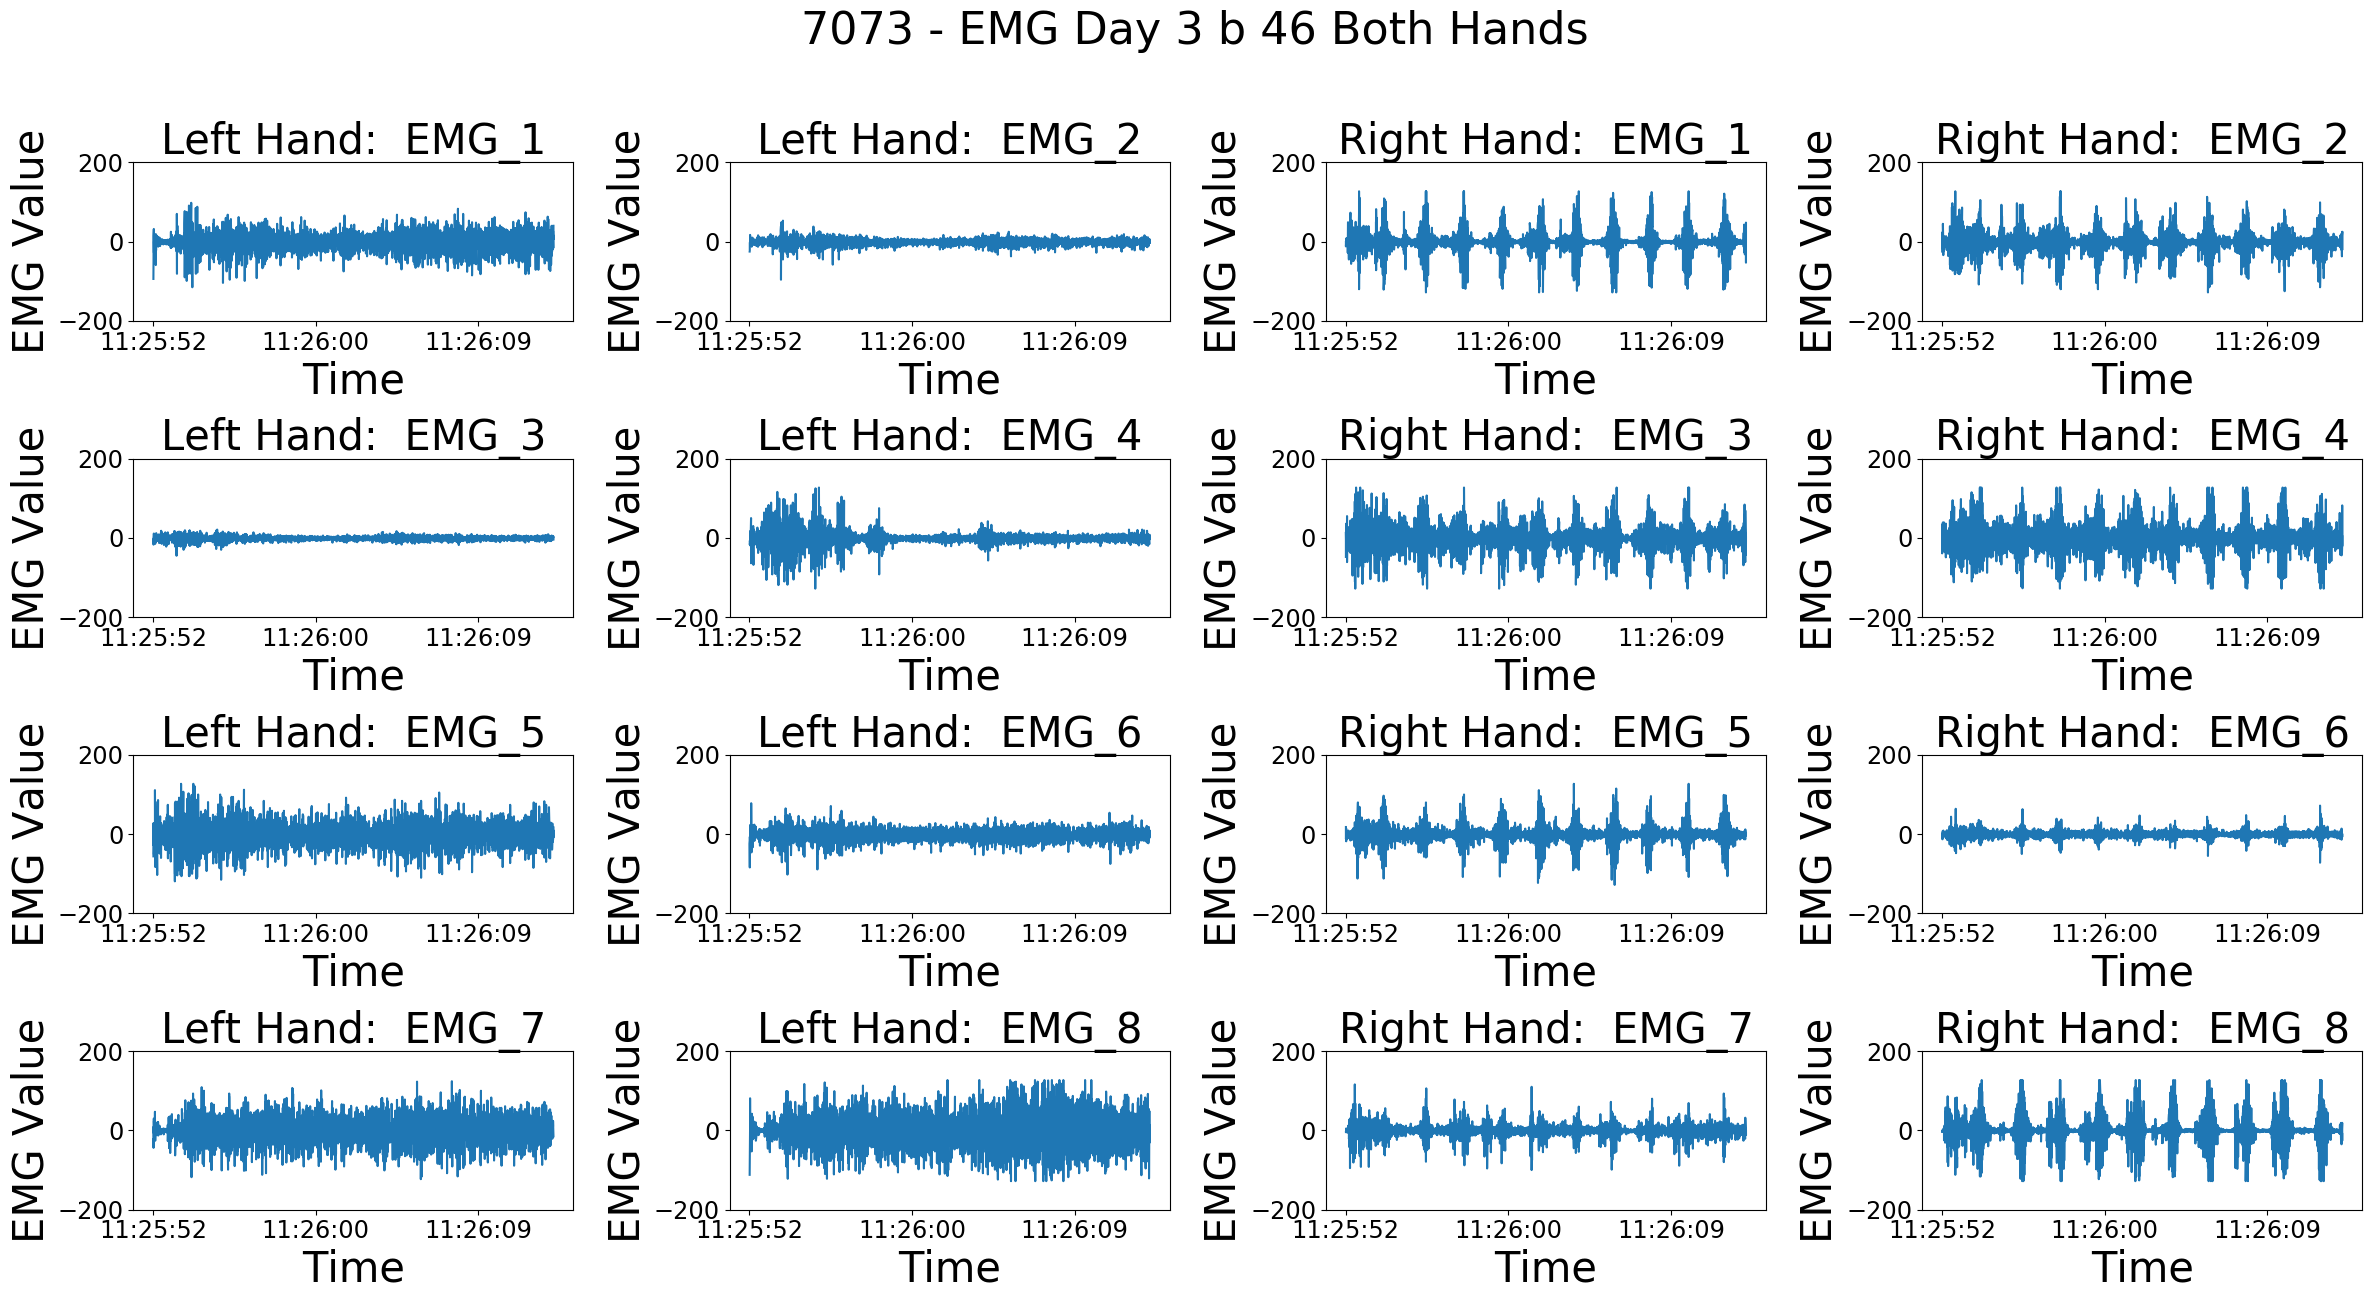
\includegraphics[width=0.8\linewidth]{pictures/7073_EMG_Day3_b_46}
	\caption{EMG data for Bag-Valve-Mask ventilation}
	\label{fig:7073emgday3b46}
\end{figure}
\begin{table}[]
	\centering
	\begin{tabular}{lllllllllllll}
		\multirow{2}{*}{\rotatebox[origin=c]{45}{\textbf{Participant}}}& \multicolumn{3}{c}{\textbf{decision-tree}} & \multicolumn{3}{c}{\textbf{$k$-NN} ($k=4$)} & \multicolumn{3}{c}{\textbf{SVM}} & \multicolumn{3}{c}{\textbf{HMM}} \\
		 & \rot{Precision}     & \rot{Recall}    & \rot{F1}    & \rot{Precision}     & \rot{Recall}    & \rot{F1}  & \rot{Precision}     & \rot{Recall}    & \rot{F1} & \rot{Precision}     & \rot{Recall}    & \rot{F1} \\
		\textbf{1}   & 0.81 & 0.48 & 0.60 & 0.67 & 0.30 & 0.41 & 0.31 & 0.19 & 0.23 & 0.50 & 0.25 & 0.33 \\
		\textbf{2}   & 0.79 & 0.78 & 0.78 & 0.58 & 0.17 & 0.27 & 0.31 & 0.23 & 0.26 & 0.90 & 0.75 & 0.82 \\
		\textbf{3}   & 0.56 & 0.54 & 0.55 & 0.32 & 0.13 & 0.18 & 0.32 & 0.26 & 0.29 & 0.88 & 0.70 & 0.78 \\
		\textbf{4}   & 0.47 & 0.45 & 0.46 & 0.27 & 0.06 & 0.10 & 0.22 & 0.20 & 0.21 & 0.71 & 0.50 & 0.59 \\
		\textbf{5}   & 0.71 & 0.58 & 0.64 & 0.11 & 0.04 & 0.05 & 0.24 & 0.25 & 0.25 & 0.86 & 0.60 & 0.71 \\
		\textbf{6}   & 0.55 & 0.50 & 0.53 & 0.33 & 0.07 & 0.12 & 0.38 & 0.29 & 0.32 & 0.60 & 0.33 & 0.43 \\
		\textbf{7}   & 0.62 & 0.63 & 0.63 & 0.28 & 0.07 & 0.12 & 0.26 & 0.24 & 0.25 & 1.00 & 0.57 & 0.73 \\
		\textbf{8}   & 0.50 & 0.52 & 0.51 & 0.18 & 0.05 & 0.08 & 0.16 & 0.14 & 0.15 & 0.57 & 0.44 & 0.50 \\
		\textbf{9}   & 0.63 & 0.59 & 0.61 & 0.33 & 0.09 & 0.14 & 0.33 & 0.35 & 0.34 & 0.80 & 0.44 & 0.57 \\
		\textbf{10} & 0.67 & 0.63 & 0.65 & 0.12 & 0.02 & 0.03 & 0.30 & 0.33 & 0.32 & 1.00 & 0.90 & 0.95 \\
		\hline
		\textbf{Mean} & 0.63 & 0.57 & 0.60 & 0.31 & 0.10 & 0.14 & 0.28 & 0.25 & 0.26 & 0.78 & 0.55 & 0.64 \\
		\textbf{Std. Dev.} & 0.12 & 0.01 & 0.09 & 0.17 & 0.08 & 0.11 & 0.07 & 0.06 & 0.06 & 0.18 & 0.20 & 0.19
	\end{tabular}
	\caption{Ten-fold cross validation for detecting BVM ventilation per participant}
	\label{tab:bvm:ml}
\end{table}
\subsection{Discussion}
\label{sec:Results:BVM:Discussion}
The Bag-Valve-Mask ventilation procedure has such a unique squeezing movement that initial assumption concluded that it would be one of the easiest procedures to detect. In contrast it turned out to be one of the hardest, which may be due to its movement overlap with CPR. The HMM classifier succeeded in achieving the highest score, possibly for the ability to detect similar sequences over periods of time.
\section{Placing Oral Airway}
\label{sec:Results:Oral-Airway}
The participants took an average of 6.51 seconds (St. Dev. = 2.23) to complete one round of the cardiopulmonary resuscitation procedure. The participants were able to complete an average of four rounds within the one minute data collection of every procedure. The amount of datasets for the third day were about 9 per participant, resulting in a total of about 90 datasets.
\par The placing an oral airway datasets consists of the unique rotating motion after the oral airway is inserted into the mouth and rotated 180 degrees. The rotating motion is visible in the right hand orientation graph in Figure \ref{fig:2334imuday3o22}. The acceleration data does not show any significant shapes of distribution. The EMG data in Figure \ref{fig:2334emgday3o22} shows a spike in channel three, four, and five when the oral airway is rotated.
\par Placing an oral airway has one of the lowest F1 scores of all procedures, with F1 scores as low as 0.00, as seen in Table \ref{tab:o:ml}. The decision-tree classifier was the algorithm with the highest mean F1 score at 0.63 (Std. Dev=0.08), followed by the HMM algorithm at 0.51 (Std. Dev=0.27).
\begin{figure}
	\centering
	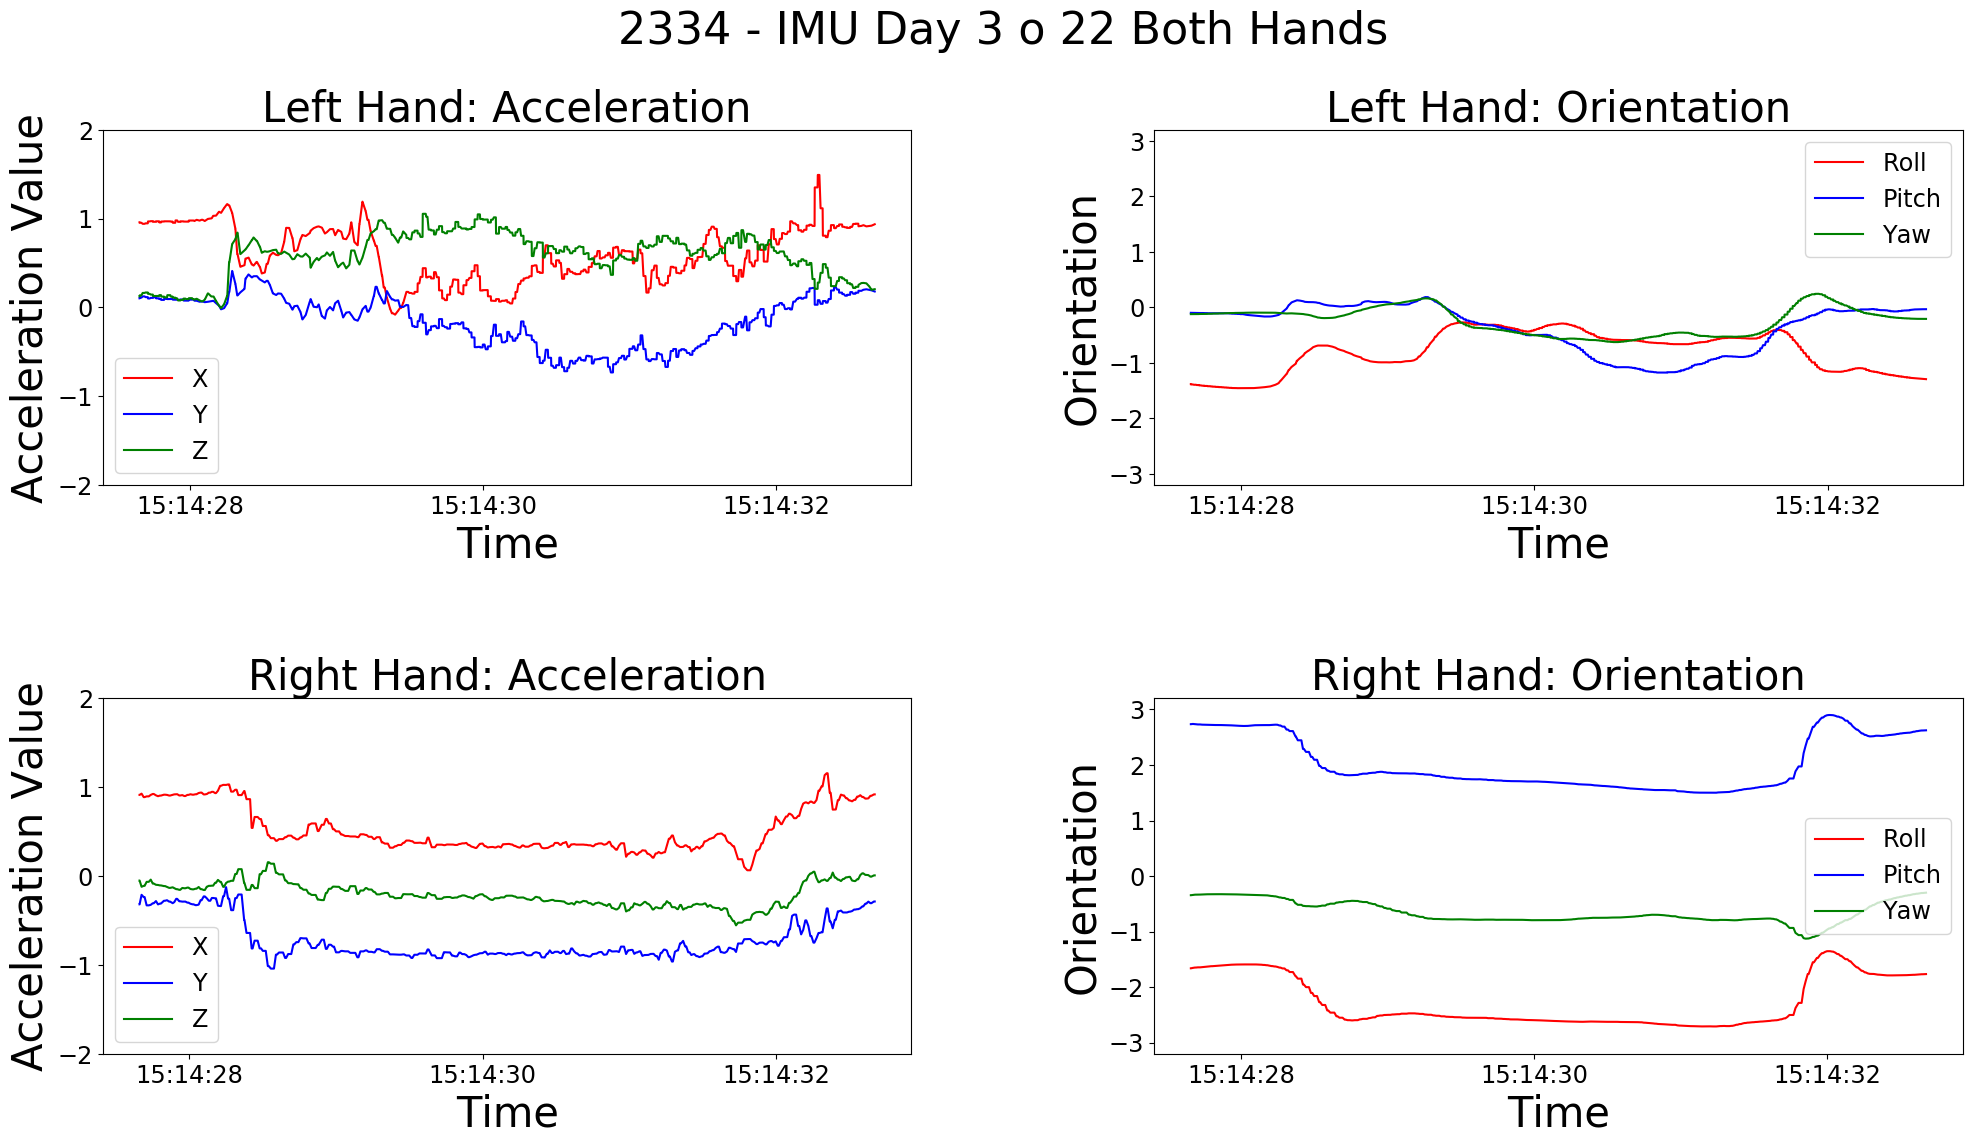
\includegraphics[width=0.8\linewidth]{pictures/2334_IMU_Day3_o_22}
	\caption{IMU data for placing an oral airway}
	\label{fig:2334imuday3o22}
\end{figure}
\begin{figure}
	\centering
	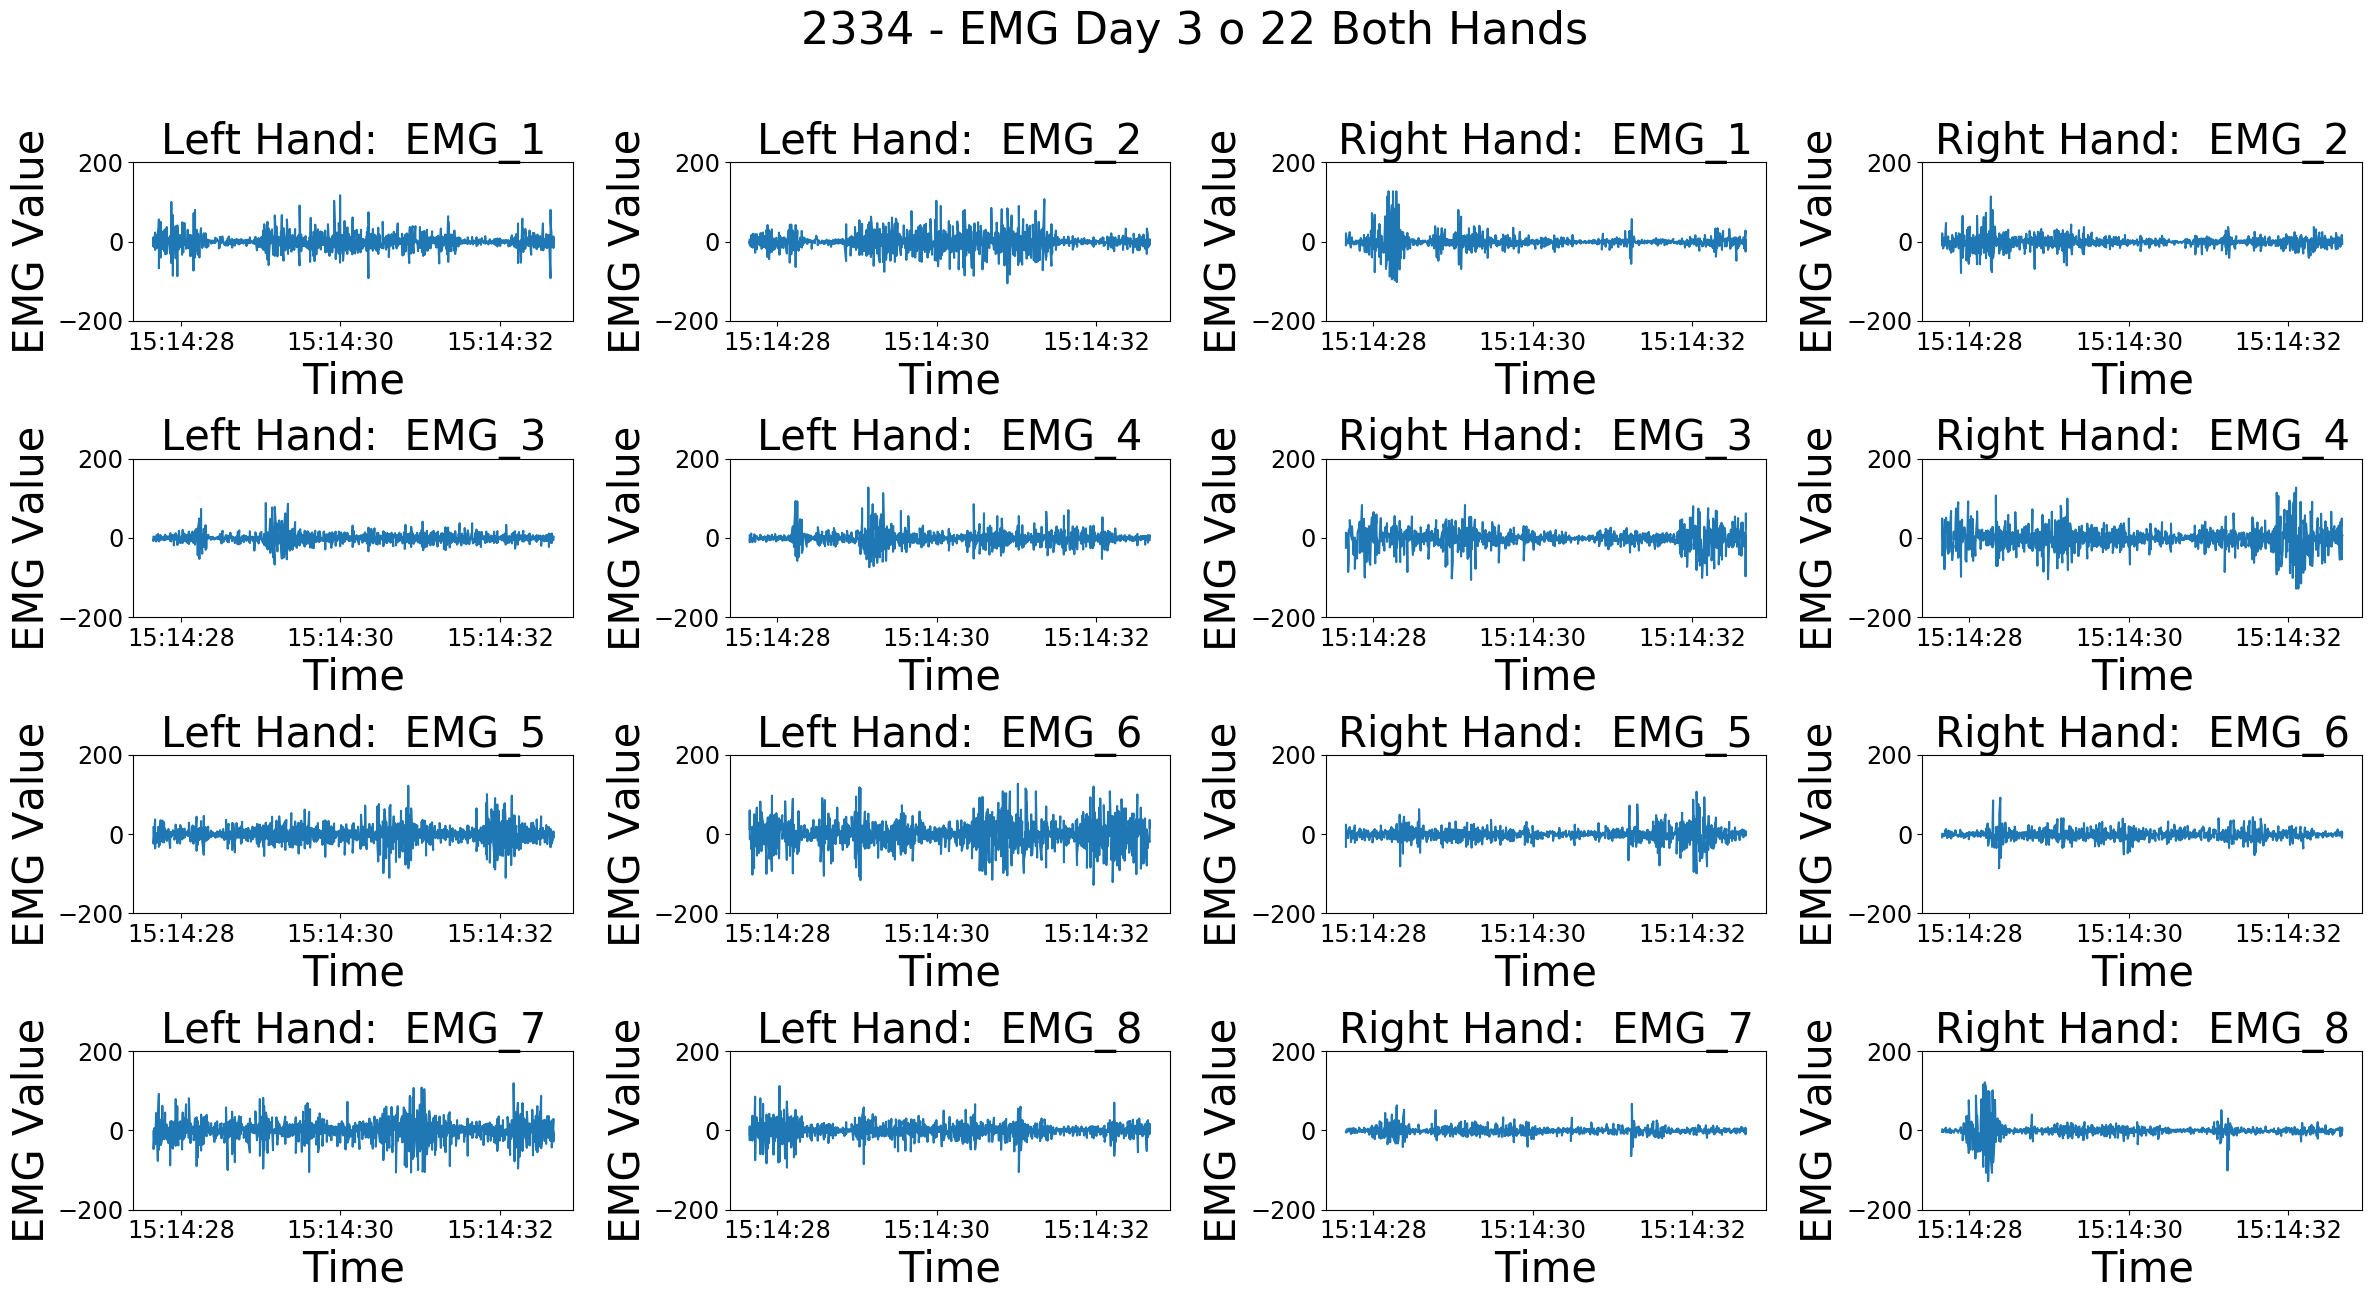
\includegraphics[width=0.8\linewidth]{pictures/2334_EMG_Day3_o_22}
	\caption{EMG data for placing an oral airway}
	\label{fig:2334emgday3o22}
\end{figure}
\begin{table}[]
	\centering
	\begin{tabular}{lllllllllllll}
		\multirow{2}{*}{\rotatebox[origin=c]{45}{\textbf{Participant}}} & \multicolumn{3}{c}{\textbf{decision-tree}} & \multicolumn{3}{c}{\textbf{$k$-NN} ($k=4$)} & \multicolumn{3}{c}{\textbf{SVM}} & \multicolumn{3}{c}{\textbf{HMM}} \\
		 & \rot{Precision}     & \rot{Recall}    & \rot{F1}    & \rot{Precision}     & \rot{Recall}    & \rot{F1}  & \rot{Precision}     & \rot{Recall}    & \rot{F1} & \rot{Precision}     & \rot{Recall}    & \rot{F1} \\
		\textbf{1}   & 0.47 & 0.58 & 0.52 & 0.26 & 0.14 & 0.18 & 0.24 & 0.18 & 0.21 & 0.00 & 0.00 & 0.00 \\
		\textbf{2}   & 0.63 & 0.56 & 0.59 & 0.29 & 0.10 & 0.15 & 0.19 & 0.21 & 0.20 & 1.00 & 0.50 & 0.67 \\
		\textbf{3}   & 0.67 & 0.76 & 0.71 & 0.50 & 0.17 & 0.25 & 0.29 & 0.24 & 0.26 & 0.78 & 0.70 & 0.74 \\
		\textbf{4}   & 0.68 & 0.65 & 0.66 & 0.44 & 0.10 & 0.17 & 0.26 & 0.21 & 0.23 & 0.86 & 0.67 & 0.75 \\
		\textbf{5}   & 0.66 & 0.66 & 0.66 & 0.00 & 0.00 & 0.00 & 0.29 & 0.17 & 0.22 & 0.62 & 0.56 & 0.59 \\
		\textbf{6}   & 0.71 & 0.71 & 0.71 & 0.27 & 0.06 & 0.10 & 0.16 & 0.15 & 0.16 & 0.75 & 0.67 & 0.71 \\
		\textbf{7}   & 0.60 & 0.59 & 0.60 & 0.12 & 0.03 & 0.05 & 0.23 & 0.18 & 0.20 & 0.50 & 0.14 & 0.22 \\
		\textbf{8}   & 0.71 & 0.78 & 0.74 & 0.38 & 0.12 & 0.19 & 0.28 & 0.20 & 0.23 & 0.25 & 0.11 & 0.15 \\
		\textbf{9}   & 0.62 & 0.66 & 0.64 & 0.09 & 0.04 & 0.05 & 0.15 & 0.11 & 0.13 & 0.80 & 0.50 & 0.62 \\
		\textbf{10} & 0.54 & 0.59 & 0.57 & 0.40 & 0.06 & 0.10 & 0.16 & 0.13 & 0.14 & 0.67 & 0.57 & 0.62 \\
		\hline
		\textbf{Mean} & 0.63 & 0.65 & 0.63 & 0.28 & 0.08 & 0.12 & 0.22 & 0.18 & 0.20 & 0.62 & 0.44 & 0.51 \\
		\textbf{Std. Dev.} & 0.08 & 0.08 & 0.08 & 0.16 & 0.05 & 0.08 & 0.06 & 0.04 & 0.04 & 0.30 & 0.26 & 0.27 \\
	\end{tabular}
	\caption{Ten-fold cross validation for detecting oral airway placement per participant}
	\label{tab:o:ml}
\end{table}
\subsection{Discussion}
\label{sec:Results:Oral-Airway:Discussion}
The F1 scores show that detecting the placement of an oral airway is challenging. The short duration for the placement does not leave much time for the algorithm to detect unique movements. The grabbing and spinning motion can occur in several other procedures when tools are picked up and put into place.
\section{Placing IV Tourniquet}
\label{sec:Results:Tourniquet}
The participants took an average of 9.38 seconds (St. Dev. = 2.70) to complete one round of the cardiopulmonary resuscitation procedure. The participants were able to complete an average of three rounds within the one minute data collection of every procedure. The amount of datasets for the third day were seven per participant, resulting in a total of 70 datasets.
\par The placing of an intravenous tourniquet consists of a single wrapping motion around the arm and tying of the ends. The wrapping and tying motion is visible in the orientation data of the IMU in Figure \ref{fig:4501imuday3t7}. The acceleration and EMG in Figure \ref{fig:4501emgday3t7} data do not show any significant distribution of data.
\par Placing an oral airway achieved good F1 for all machine learning algorithms except the HMM algorithm, as seen in Table \ref{tab:t:ml}. The decision-tree classifier was the algorithm with the highest mean F1 score at 0.81 (Std. Dev=0.06), followed by the SVM algorithm at 0.53 (Std. Dev=0.10). The HMM algorithm came last with a F1 score of 0.24 (Std. Dev=0.21).
\begin{figure}
	\centering
	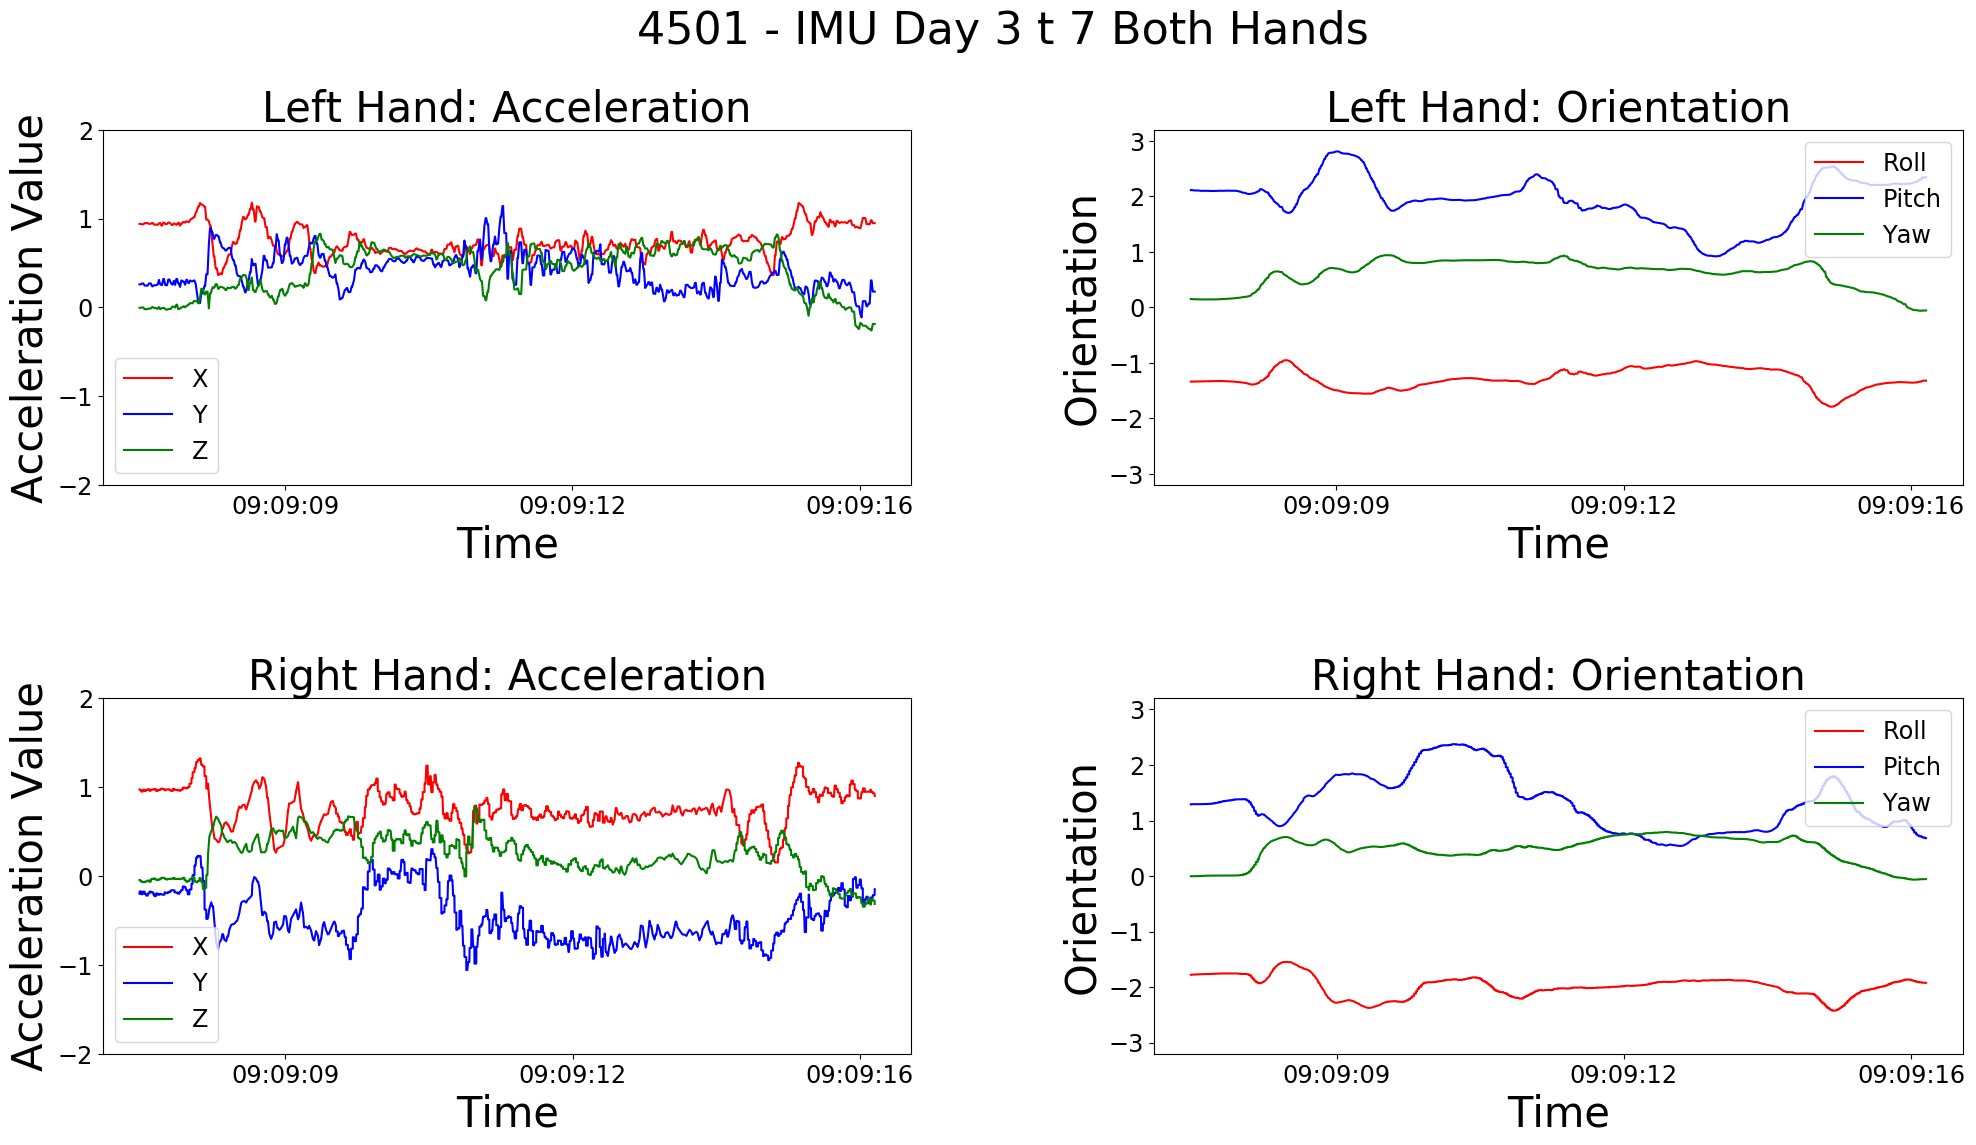
\includegraphics[width=0.8\linewidth]{pictures/4501_IMU_Day3_t_7}
	\caption{IMU data for placing an IV tourniquet}
	\label{fig:4501imuday3t7}
\end{figure}
\begin{figure}
	\centering
	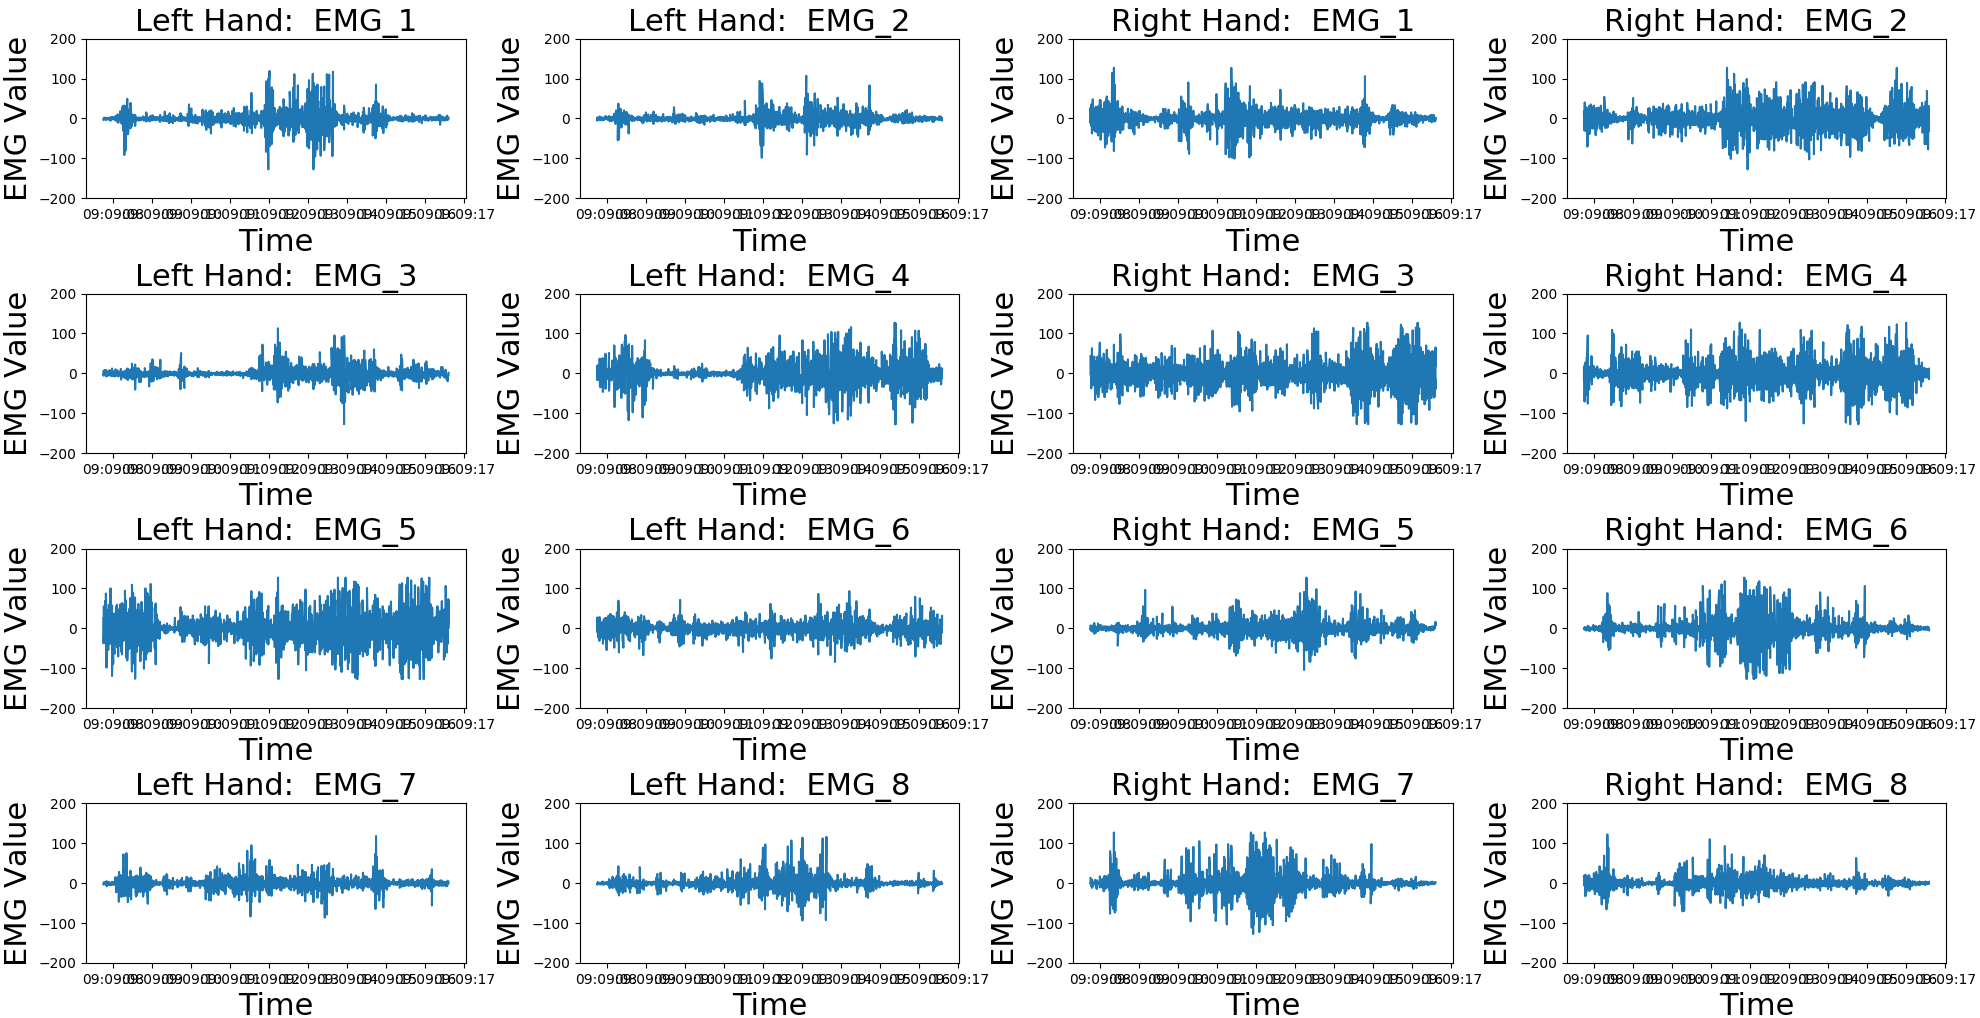
\includegraphics[width=0.8\linewidth]{pictures/4501_EMG_Day3_t_7}
	\caption{EMG data for placing an IV tourniquet}
	\label{fig:4501emgday3t7}
\end{figure}
\begin{table}[]
	\centering
	\begin{tabular}{lllllllllllll}
		\multirow{2}{*}{\rotatebox[origin=c]{45}{\textbf{Participant}}} & \multicolumn{3}{c}{\textbf{decision-tree}} & \multicolumn{3}{c}{\textbf{$k$-NN} ($k=4$)} & \multicolumn{3}{c}{\textbf{SVM}} & \multicolumn{3}{c}{\textbf{HMM}} \\
		 & \rot{Precision}     & \rot{Recall}    & \rot{F1}    & \rot{Precision}     & \rot{Recall}    & \rot{F1}  & \rot{Precision}     & \rot{Recall}    & \rot{F1} & \rot{Precision}     & \rot{Recall}    & \rot{F1} \\
		\textbf{1}   & 0.65 & 0.65 & 0.65 & 0.30 & 0.36 & 0.33 & 0.29 & 0.30 & 0.30 & 0.22 & 0.40 & 0.29 \\
		\textbf{2}   & 0.80 & 0.81 & 0.80 & 0.31 & 0.56 & 0.40 & 0.51 & 0.62 & 0.56 & 0.00 & 0.00 & 0.00 \\
		\textbf{3}   & 0.83 & 0.81 & 0.82 & 0.30 & 0.57 & 0.39 & 0.43 & 0.56 & 0.49 & 0.00 & 0.00 & 0.00 \\
		\textbf{4}   & 0.84 & 0.85 & 0.84 & 0.37 & 0.64 & 0.47 & 0.56 & 0.67 & 0.61 & 0.50 & 0.17 & 0.25 \\
		\textbf{5}   & 0.85 & 0.87 & 0.86 & 0.34 & 0.64 & 0.45 & 0.54 & 0.71 & 0.61 & 0.00 & 0.00 & 0.00 \\
		\textbf{6}   & 0.83 & 0.80 & 0.82 & 0.31 & 0.42 & 0.36 & 0.48 & 0.59 & 0.53 & 0.33 & 0.17 & 0.22 \\
		\textbf{7}   & 0.80 & 0.79 & 0.80 & 0.27 & 0.44 & 0.33 & 0.42 & 0.55 & 0.48 & 0.22 & 0.33 & 0.27 \\
		\textbf{8}   & 0.89 & 0.86 & 0.87 & 0.33 & 0.60 & 0.43 & 0.50 & 0.66 & 0.57 & 0.60 & 0.50 & 0.55 \\
		\textbf{9}   & 0.80 & 0.78 & 0.79 & 0.34 & 0.53 & 0.41 & 0.47 & 0.59 & 0.53 & 0.75 & 0.50 & 0.60 \\
		\textbf{10} & 0.80 & 0.84 & 0.82 & 0.28 & 0.52 & 0.37 & 0.43 & 0.53 & 0.58 & 0.25 & 0.17 & 0.20 \\
		\hline
		\textbf{Mean} & 0.81 & 0.81 & 0.81 & 0.32 & 0.52 & 0.40 & 0.46 & 0.60 & 0.53 & 0.30 & 0.22 & 0.24 \\
		\textbf{Std. Dev.} & 0.06 & 0.06 & 0.06 & 0.03 & 0.10 & 0.05 & 0.08 & 0.11 & 0.10 & 0.26 & 0.20 & 0.21
	\end{tabular}
	\caption{Ten-fold cross validation for detecting tourniquet placement per participant}
	\label{tab:t:ml}
\end{table}
\subsection{Discussion}
\label{sec:Results:Tourniquet:Discussion}
Placing a tourniquet is one of the two short procedures with placing an oral airway. Yet it the decision-tree algorithm was able to achieve a high F1 score of 0.81. In contrast the HMM algorithm under performed with only 0.21. The low score of the HMM algorithm can be a result of a close log probability of the HMM models.
\section{Wrapping Head Wound}
\label{sec:Results:Wound}
The participants took an average of 37.26 seconds (St. Dev. = 11.72) to complete one round of the cardiopulmonary resuscitation procedure. The participants were able to complete two rounds within the one minute data collection of every procedure. The amount of datasets for the third day were seven per participant, resulting in a total of 70 datasets.
\par The wrapping of a head wound consists of the unique wrapping of a bandage around the head of a patient. The wrapping motion is primarily visible in the orientation data of the IMU in Figure \ref{fig:2334imuday3w47}. The spikes in the orientation data are sinusoidal and represent the amount of rotations around the head. The EMG data in Figure \ref{fig:2334emgday3w47} shows a lot of activity related to the grabbing and releasing of the bandage when wrapping around the patient's head.
\par Wrapping a head wound achieved the highest F1 for the decision-tree algorithm, as seen in Table \ref{tab:w:ml}. The decision-tree classifier had a mean F1 score of 0.90 (Std. Dev=0.06), followed by the SVM algorithm at 0.61 (Std. Dev=0.04). The HMM algorithm came last with a F1 score of 0.40 (Std. Dev=0.18)
\begin{figure}
	\centering
	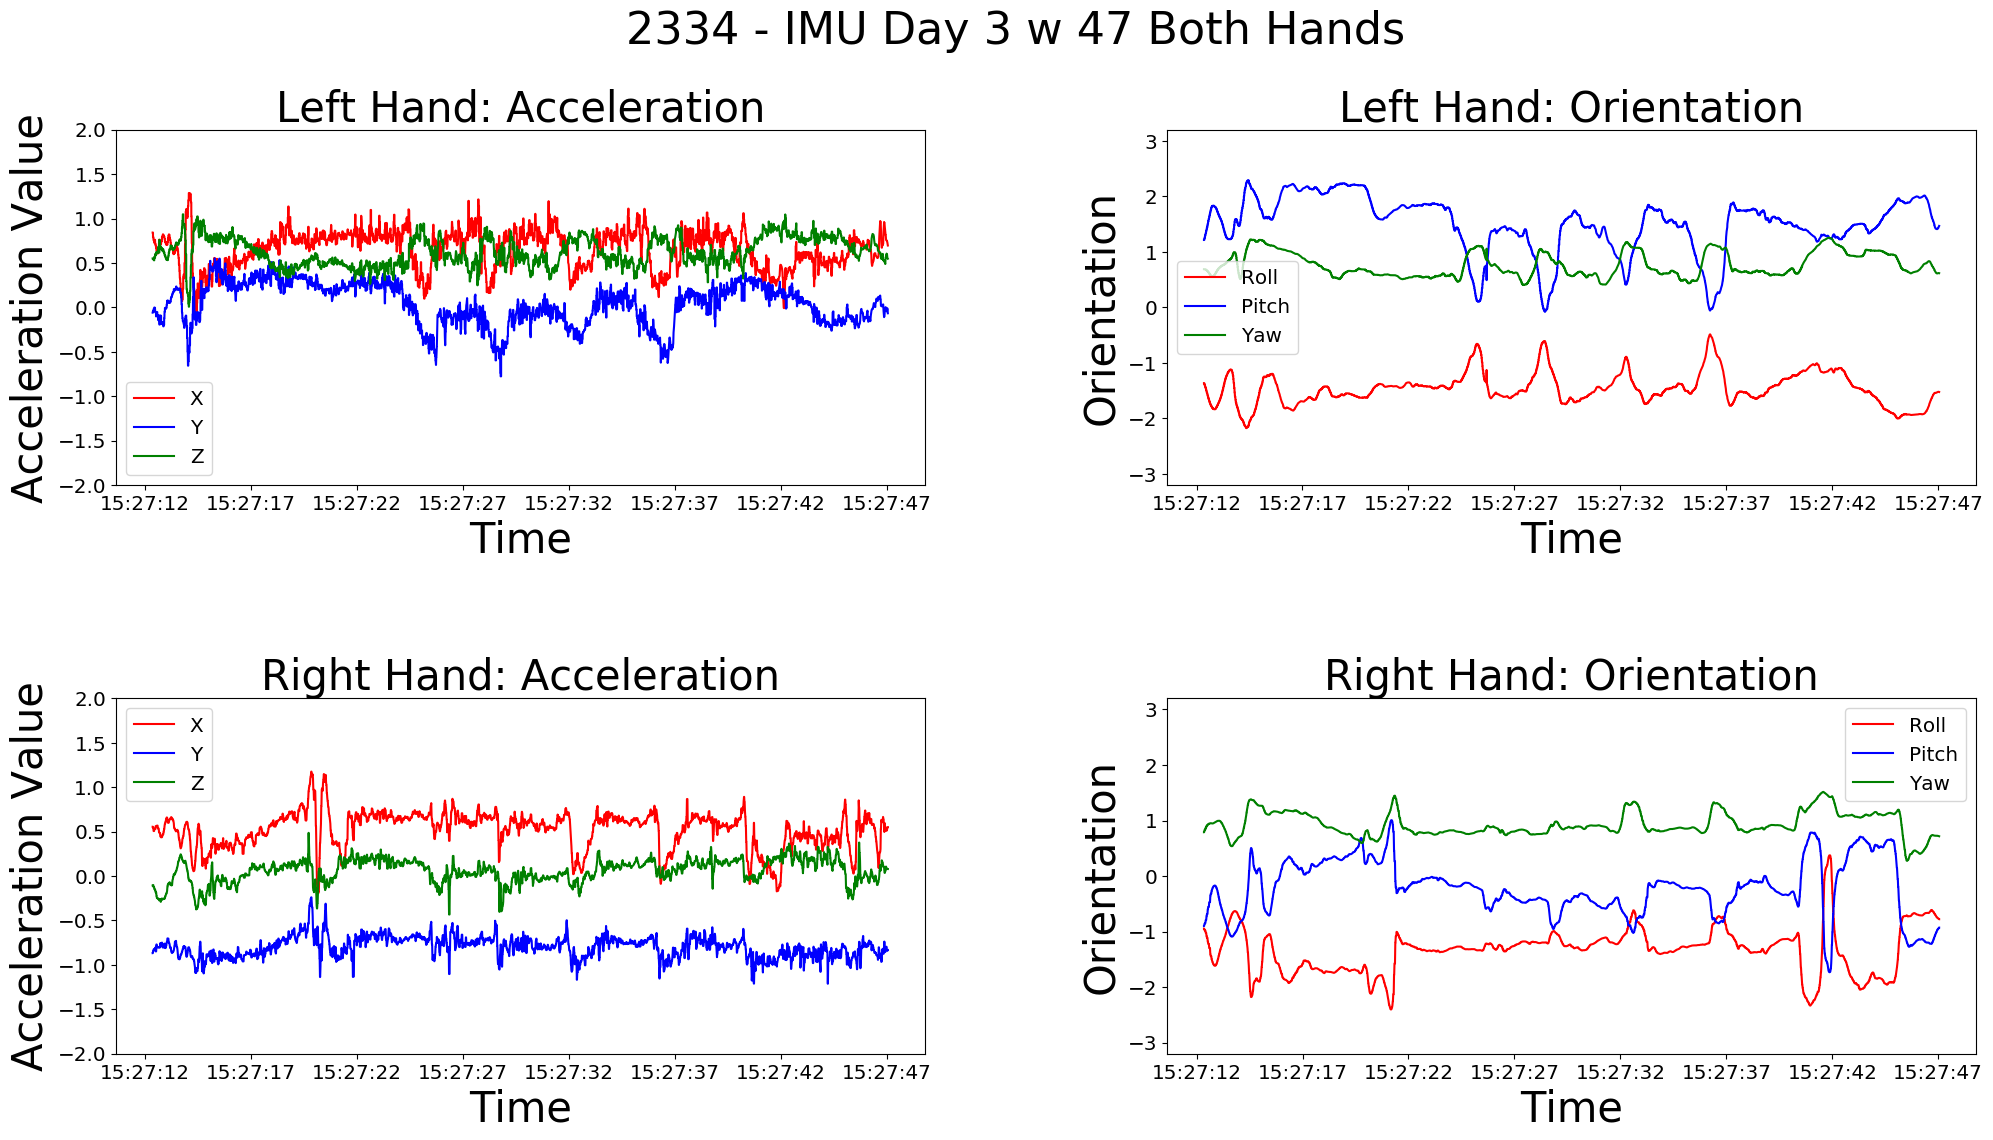
\includegraphics[width=0.8\linewidth]{pictures/2334_IMU_Day3_w_47}
	\caption{IMU data for wrapping a head wound}
	\label{fig:2334imuday3w47}
\end{figure}
\begin{figure}
	\centering
	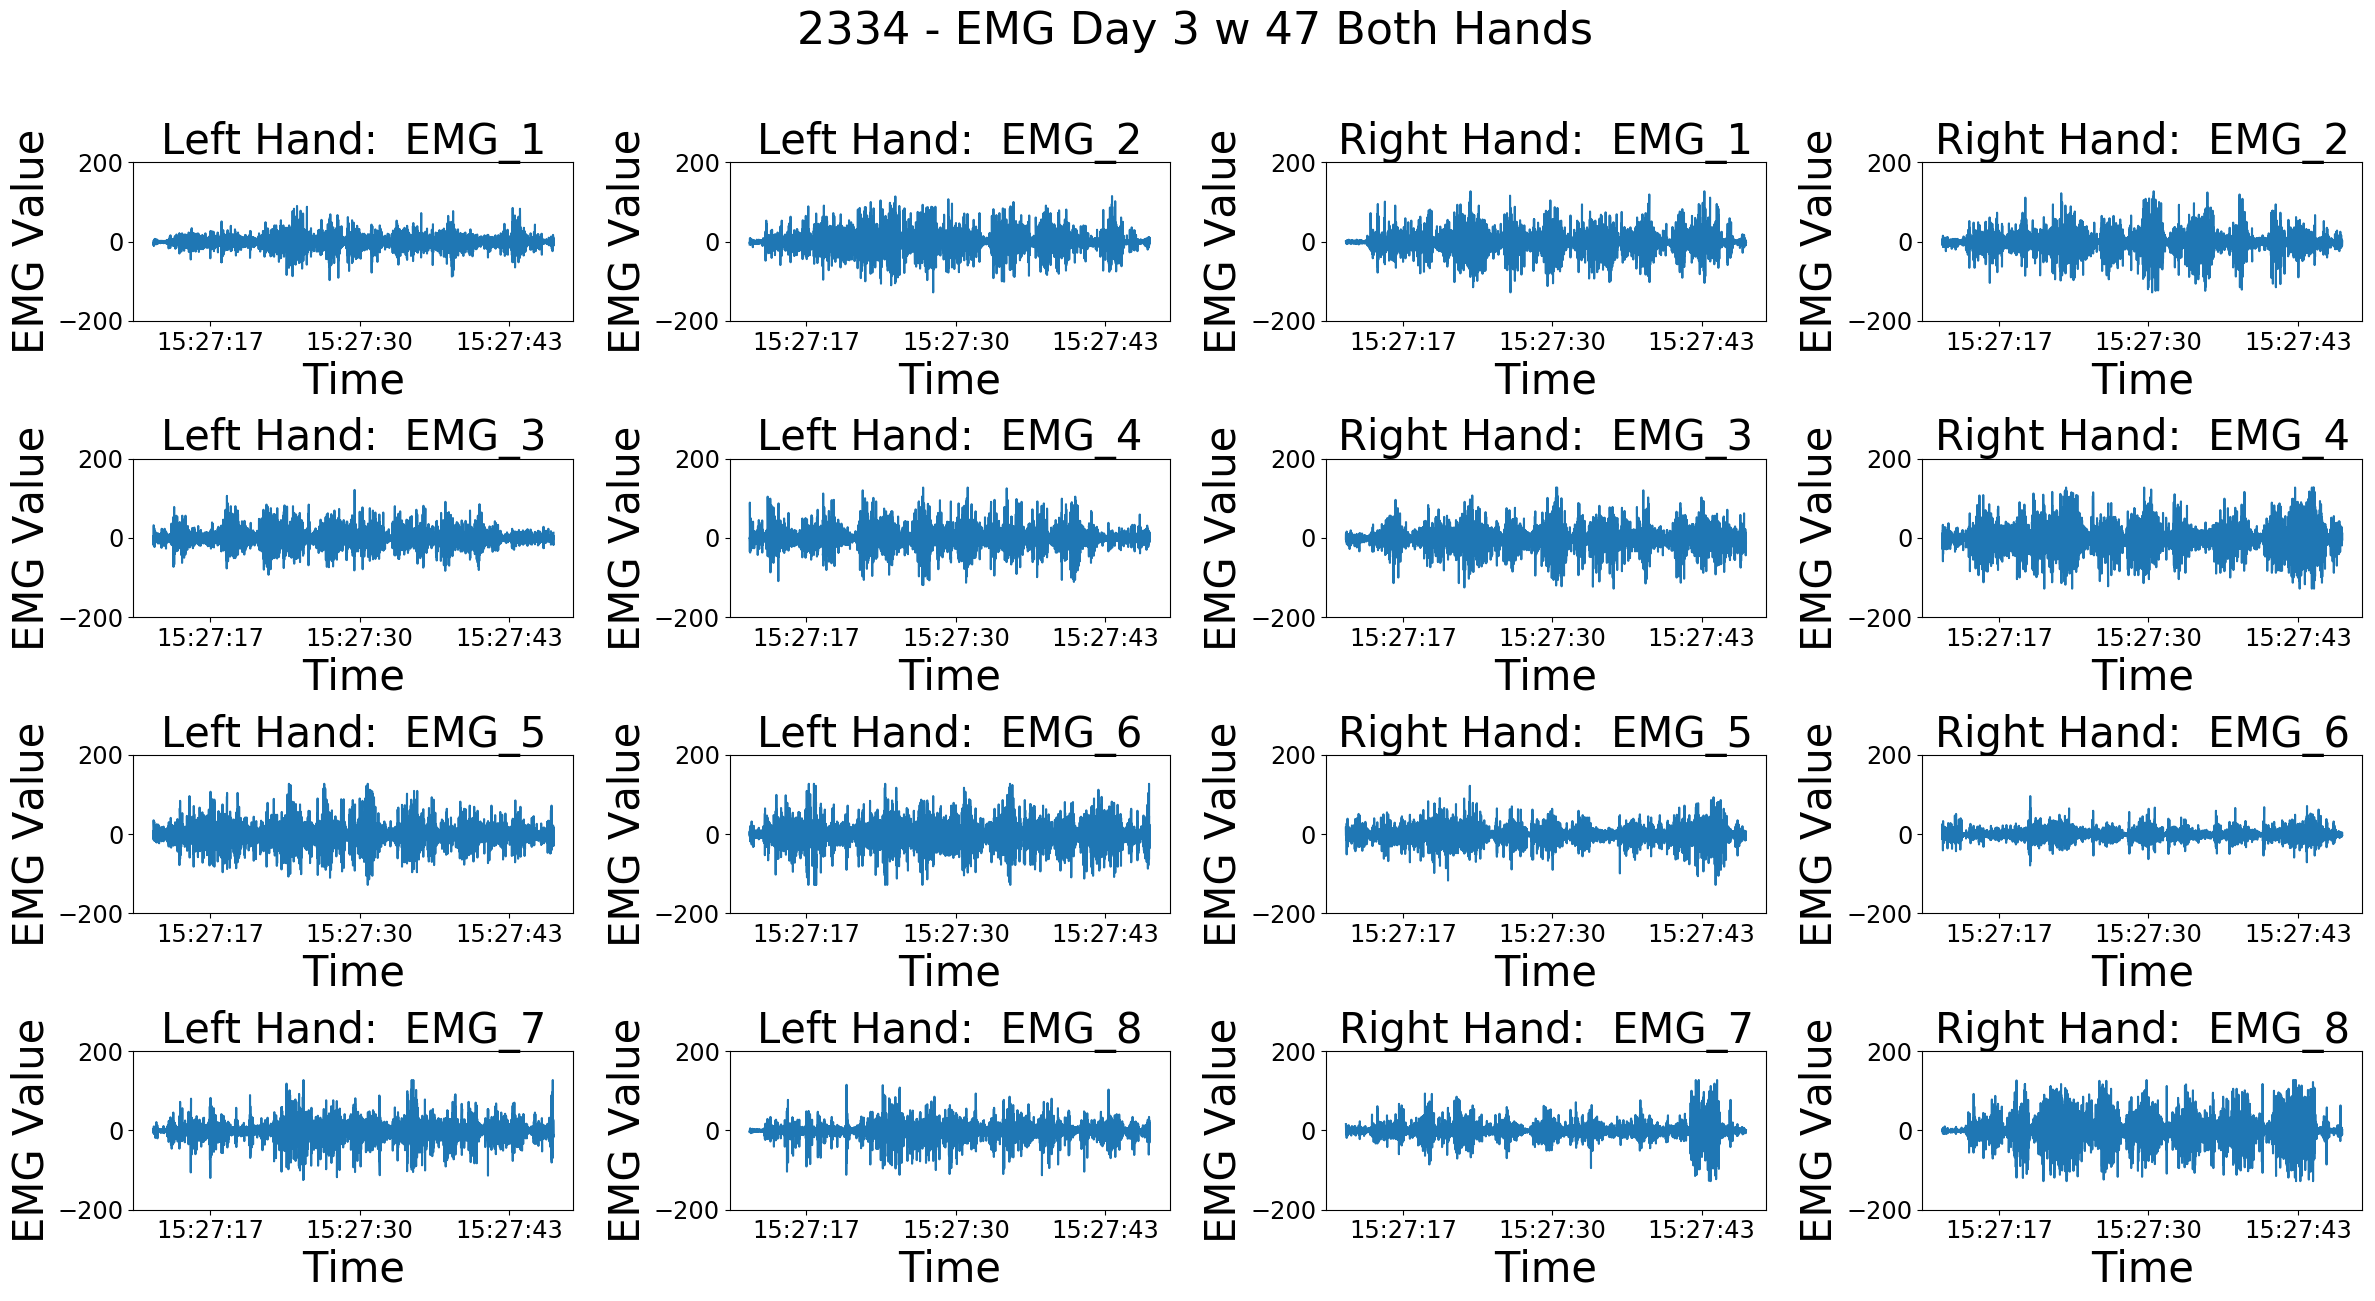
\includegraphics[width=0.8\linewidth]{pictures/2334_EMG_Day3_w_47}
	\caption{EMG data for wrapping a head wound}
	\label{fig:2334emgday3w47}
\end{figure}
\begin{table}[]
	\centering
	\begin{tabular}{lllllllllllll}
		\multirow{2}{*}{\rotatebox[origin=c]{45}{\textbf{Participant}}} & \multicolumn{3}{c}{\textbf{decision-tree}} & \multicolumn{3}{c}{\textbf{$k$-NN} ($k=4$)} & \multicolumn{3}{c}{\textbf{SVM}} & \multicolumn{3}{c}{\textbf{HMM}} \\
		 & \rot{Precision}     & \rot{Recall}    & \rot{F1}    & \rot{Precision}     & \rot{Recall}    & \rot{F1}  & \rot{Precision}     & \rot{Recall}    & \rot{F1} & \rot{Precision}     & \rot{Recall}    & \rot{F1} \\
		\textbf{1}   & 0.73 & 0.72 & 0.72 & 0.43 & 0.54 & 0.48 & 0.47 & 0.66 & 0.55 & 0.20 & 0.20 & 0.20 \\
		\textbf{2}   & 0.88 & 0.91 & 0.89 & 0.45 & 0.46 & 0.46 & 0.60 & 0.58 & 0.59 & 0.30 & 0.50 & 0.37 \\
		\textbf{3}   & 0.81 & 0.83 & 0.82 & 0.42 & 0.42 & 0.42 & 0.63 & 0.62 & 0.62 & 0.38 & 0.83 & 0.53 \\
		\textbf{4}   & 0.91 & 0.90 & 0.90 & 0.43 & 0.49 & 0.46 & 0.61 & 0.63 & 0.62 & 0.22 & 0.33 & 0.27 \\
		\textbf{5}   & 0.87 & 0.87 & 0.87 & 0.42 & 0.39 & 0.40 & 0.63 & 0.63 & 0.63 & 0.29 & 0.33 & 0.31 \\
		\textbf{6}   & 0.88 & 0.90 & 0.89 & 0.45 & 0.65 & 0.53 & 0.54 & 0.55 & 0.55 & 0.44 & 0.67 & 0.53 \\
		\textbf{7}   & 0.92 & 0.91 & 0.92 & 0.49 & 0.54 & 0.51 & 0.60 & 0.65 & 0.62 & 0.00 & 0.00 & 0.00 \\
		\textbf{8}   & 0.94 & 0.92 & 0.93 & 0.43 & 0.48 & 0.45 & 0.62 & 0.59 & 0.61 & 0.25 & 0.50 & 0.33 \\
		\textbf{9}   & 0.88 & 0.90 & 0.89 & 0.49 & 0.55 & 0.51 & 0.68 & 0.68 & 0.68 & 0.45 & 0.83 & 0.59 \\
		\textbf{10} & 0.92 & 0.93 & 0.93 & 0.44 & 0.51 & 0.47 & 0.66 & 0.67 & 0.67 & 0.38 & 0.50 & 0.43 \\
		\hline
		\textbf{Mean} & 0.90 & 0.90 & 0.90 & 0.44 & 0.50 & 0.50 & 0.60 & 0.63 & 0.61 & 0.30 & 0.50 & 0.40 \\
		\textbf{Std. Dev.} & 0.06 & 0.06 & 0.06 & 0.03 & 0.07 & 0.04 & 0.06 & 0.04 & 0.04 & 0.13 & 0.30 & 0.18
	\end{tabular}
	\caption{Ten-fold cross validation for detecting wrapping a wound per participant}
	\label{tab:w:ml}
\end{table}
\subsection{Discussion}
\label{sec:Results:Wound:Discussion}
The repeated wrapping motion of bandaging a head wound resulted in the highest score for the decision-tree algorithm. The HMM algorithm under performed at detecting the procedure and had the highest standard deviation. Participant three, six, and nine had the highest F1 score across all machine learning algorithms. Participant seven achieved 0.92 for the decision-tree algorithm, but 0.00 for the HMM algorithm. The wide gap between recognition score can be contributed to the problem the HMM algorithm has with picking the best model given the log probabilities.
\section{Generalizability}
\label{sec:Results:Generalizability}
The datasets of all participants is combined to create one large dataset. The F1 score is a bit lower when comparing the machine learning algorithms on the combined dataset to the individual participants. The highest F1 score on the combined dataset is achieved by the decision-tree algorithm with 0.71, as shown in Table \ref{tab:ml}. The HMM algorithm followed second with 0.44, then $k$-NN with 0.35, and last the SVM with 0.25.
\begin{table}[]
	\centering
	\begin{tabular}{llllllllllll}
		\multicolumn{3}{c}{\textbf{decision-tree}} & \multicolumn{3}{c}{\textbf{$k$-NN} ($k=4$)} & \multicolumn{3}{c}{\textbf{SVM}} & \multicolumn{3}{c}{\textbf{HMM}} \\
		\rot{Precision}     & \rot{Recall}    & \rot{F1}    & \rot{Precision}     & \rot{Recall}    & \rot{F1}  & \rot{Precision}     & \rot{Recall}    & \rot{F1} & \rot{Precision}     & \rot{Recall}    & \rot{F1} \\
		0.71 & 0.71 & 0.71 & 0.37 & 0.37 & 0.35 & 0.42 & 0.39 & 0.25 & 0.47 & 0.44 & 0.44 \\
	\end{tabular}
	\caption{Ten-fold cross validation for detecting every procedure}
	\label{tab:ml}
\end{table}
\subsection{Discussion}
\label{sec:Results:Generalizability:Discussion}
The combined dataset allowed the machine learning algorithms to train on several participants, each with different approaches to the procedures. The unique movements may all look similar, the way participants grab and adjust tools can be different. Figure \ref{fig:5187emgday3t1average} shows the average of all participants in red. Similarities between the average EMG data and the data of the participant can be seen, yet some noise is observable in channels three, four, and five.
\begin{figure}
	\centering
	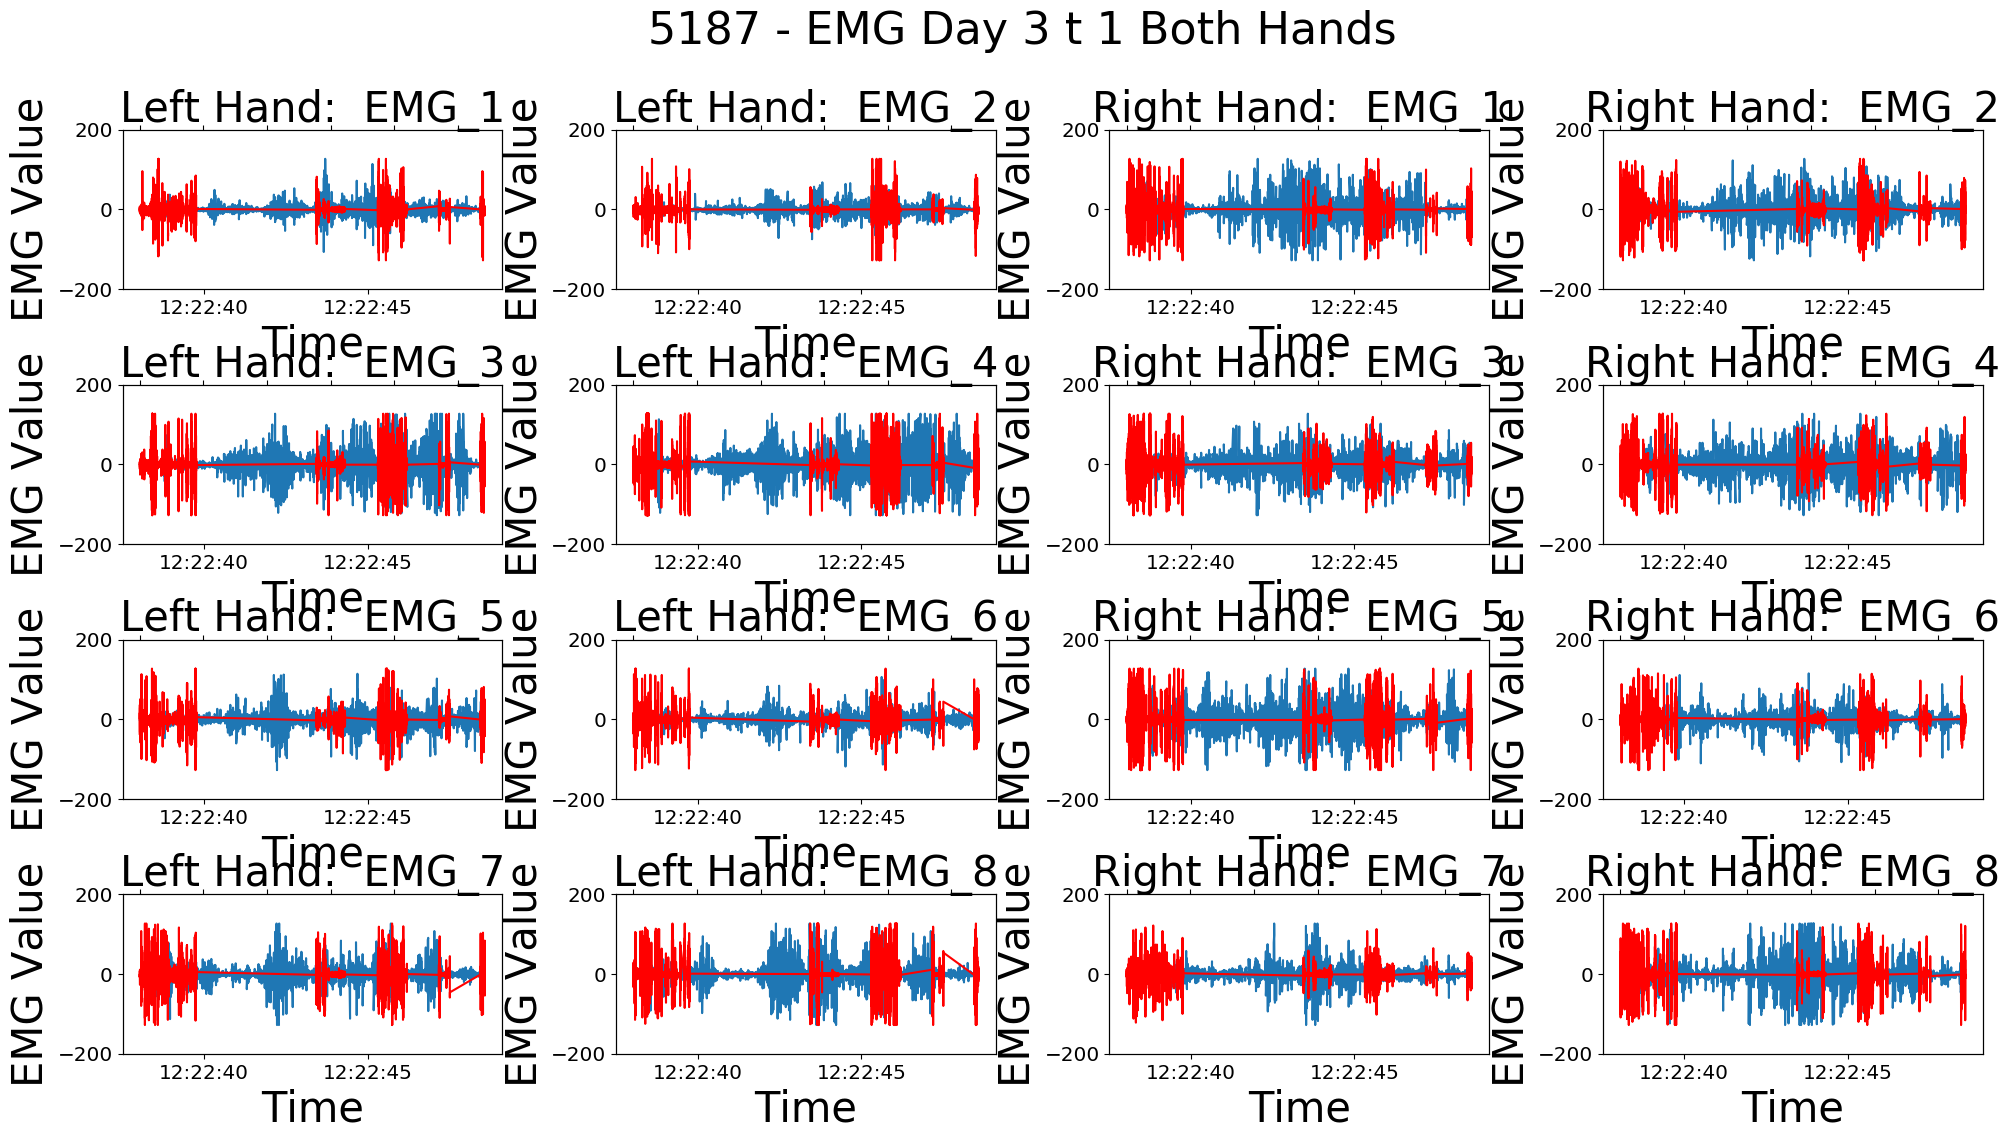
\includegraphics[width=0.7\linewidth]{pictures/5187_EMG_Day3_t_1_average}
	\caption{Tourniquet EMG data with average in red}
	\label{fig:5187emgday3t1average}
\end{figure}

\section{Discussion}
\label{sec:Results:Discussion}
Research question $H_1$ proposed that CPR and bag-valve-mask ventilation have the highest recognition accuracy compared to the other procedures. Comparing the F1 score of the decision-tree classifier CPR and bag-valve-mask ventilation received 0.83 and 0.60 respectively. Oral airway achieved 0.63, IV tourniquet 0.81, and wrapping a wound 0.90. Wrapping a wound achieved the highest score, followed by CPR. Bag-valve-mask ventilation received the lowest score. Contrary to the initial assumption, the unique movements during CPR were not as helpful to accuracy detect the procedure as predicted. The overlap of the giving breaths motion resulted in high misclassification as Bag-Valve-Mask ventilation. Figure \ref{fig:knn46s} shows the confusion matrix for the generalized $k$-NN ($k=4$) algorithm with a window size of 6 seconds. CPR, bag-valve-mask ventilation, and wrapping a wound were missclassified within eachother several times.
\begin{figure}
	\centering
	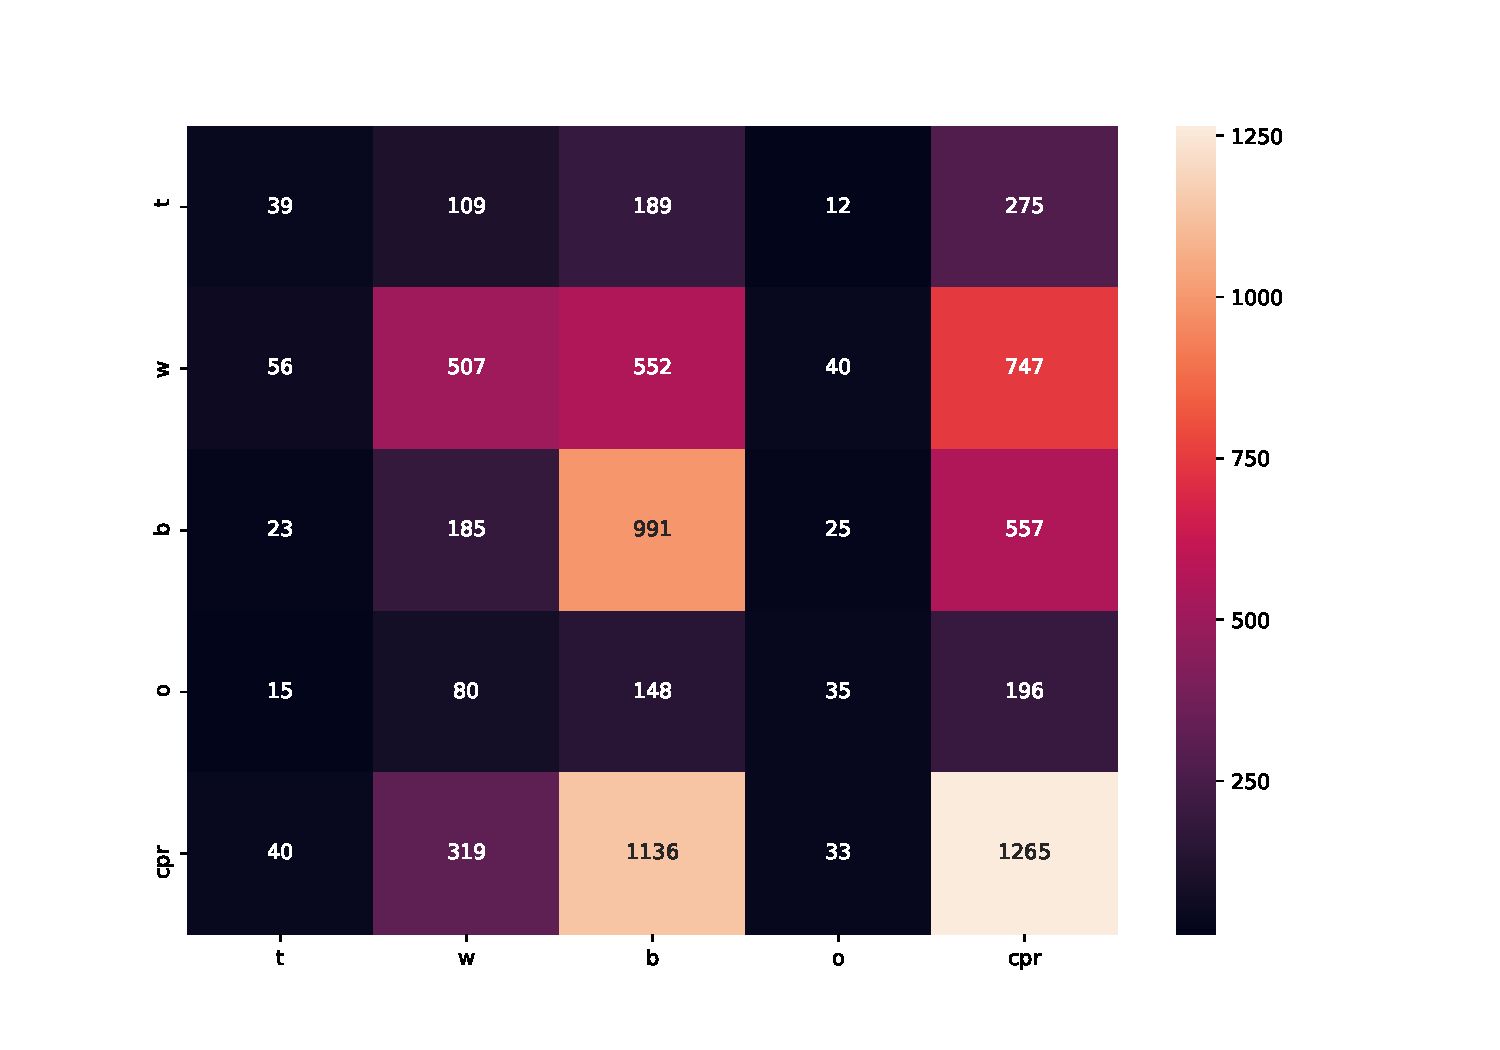
\includegraphics[width=0.7\linewidth]{pictures/knn4_6s}
	\caption{Confusion matrix for $k$-NN ($k=4$) algorithm}
	\label{fig:knn46s}
\end{figure}
\par The decision-tree algorithm was the highest scoring machine learning algorithm. The HMM algorithm placed second close to $k$-NN ($k=4$). Research question $H_2$ assumed the HMM algorithm to be the most accurate machine learning algorithm, due to its ability to take sequences of data. Overfitting for the decision-tree algorithm is a potential problem, but the decision-tree algorithm was able to maintain a high F1 score when using the combined dataset.

